\documentclass[11pt,a4paper]{article}

\setlength{\parskip}{\baselineskip}%
\setlength{\parindent}{0pt}%
\usepackage[english]{babel}
\usepackage[utf8]{inputenc}
\usepackage{amsmath}
\usepackage{graphicx}
\usepackage[colorinlistoftodos]{todonotes}
\usepackage{float}
\usepackage[top=1.1in, bottom=1.1in, left=1.2in, right=1.2in]{geometry}
\usepackage{listings} 
\lstset{
        language=Matlab,
        breaklines=true
    }
\usepackage{url}
\usepackage{lipsum}
\usepackage{wrapfig}
\usepackage{fancyhdr}
\usepackage{caption}
\usepackage{subcaption}
\usepackage{multirow}
\usepackage[none]{hyphenat}
\usepackage[framed,numbered,autolinebreaks,useliterate]{mcode}
\pagestyle{fancy}
\lhead{FOVEROS Chess Engine}
\rhead{\thepage}
\cfoot{}
\renewcommand{\headrulewidth}{0.8pt}
\renewcommand{\footrulewidth}{0.8pt}
\lstset{breakatwhitespace=false}
\graphicspath{ {./Pictures/} }
\begin{document}


\begin{titlepage}

\title{\huge  FOVEROS Chess Engine\\\Large (Modelling 2)}
\author{\Large Lim, Ji Xiong\\Student no: 1327879\\Candidate no: 61135\and \Large Variath Paul, Joel\\Student no: 1352347\\Candidate no: 62790}
\date{\parbox{\linewidth}{\centering%
  \Large\today\endgraf\bigskip\medskip
  Department of Mechanical Engineering \endgraf
  University of Bristol}}
\maketitle
\thispagestyle{empty}


\begin{abstract}
The FOVEROS Chess Engine project is an engine built in MATLAB that encompasses the interaction, display, legality and computer thought for a chess game. A brute force approach is taken to produce computer thought using tree-search methods, MiniMax algorithm and Alpha Beta Pruning optimisation. The optimisation has shown to reduce the time taken by 90\%. A heuristic function was created to evaluate the board for the purposes of selecting the best path. 
\newline
\newline
\indent This Chess Engine successfully runs with minimal issues and demonstrates interesting characteristics such as aggression, the ability to checkmate, to castle and to evade check. The implementation of the rules of chess is near perfect and is able to execute special moves such as En Passant, Pawn Promotion and Castling.
\end{abstract}

\end{titlepage}



\setcounter{page}{2}
\tableofcontents



\newpage
\section{Introduction}

\setlength{\parindent}{6ex}
\indent\indent The history of chess spans several centuries back to India, where it is believed to have originated in the 6th century. Chess in its current form came into being around the early 1500’s. With the rise of modern technology, chess is naturally the game of choice to demonstrate the implications of increased processing power in computers. 

Chess has fascinated game theorists because it is deterministic which means that there can only be 1 winning side. It is also a game of perfect information, meaning that all the information is available to the player to make the best decision to move. This adversarial game also has well defined and rigid rules which limit movements to a relatively small number making it ideal for modelling.\cite{chess1}
 
With the development of early computers in 1950’s, the race was on to develop the ultimate chess engine that would never be beaten by a human player. Alan Turing wrote the first ever computer chess game in 1950. In 1996, Deep Blue won a match against Garry Kasparov. It was the first time a chess engine had beaten a reigning world champion.
 
Chess engines adopt a brute for approach. Therefore, development of chess engines tie together a broad range of topics, improve the understanding of tree searching algorithms and its optimisations, logical thought processes behind the game as well as a deeper understanding of computational thought and Artificial Intelligence(AI).



\newpage
\section{Modelling Aims}

\begin{enumerate}
\item To create a program that displays a standard chessboard, where the user is able move the pieces legally.
\item The program should be able to generate all possible future moves up to a specified depth using the brute force approach.
\item The user must be able to specify game settings such as: 

\begin{itemize}
\item Difficulty - Random, Easy and Hard
\item Player choice - Player Vs Player, Player Vs AI and AI Vs AI
\end{itemize}

\item The program must incorporate an algorithm that evaluates the chessboard from a certain player’s perspective to aid the AI’s decision.
\item The program must display game messages, time taken to execute moves, player scores and a player performance graph.
\end{enumerate}


\newpage
\section{Overview}
\indent\indent The architecture of the system is split into 2 parts, the frontend and the backend. The frontend consists of the Mdp\_Chessboard package provided to us which is the basis for the board graphics that is displayed. The frontend initialises a structured variable called B which contains info about the game as well as a 16 by 16 matrix that portrays the location of the chessboard pieces as the game progresses. 
\\*\\
\indent The backend consists of 3 important variables that are initialised at the start of the game which are $chessboard$, $piece\_colour$, $num\_moves$. These are all 8 by 8 matrices that display the pieces as numbers and their relevant information. All manipulation and board calculations are carried out on the backend. The calculations of possible moves that can be made are also done in the backend.
\\*\\
\indent Communication between the backend and frontend occurs through a function called $readchessboard$. This function interprets the backend variables and creates a new B that represents the backend which is ready to be plotted.
\\*\\
\indent The reason why the backend variables was used in calculations rather than $B$ is because B is a structure and contains extra information which would be unnecessary for calculation and would slow the system down.
\\*\\
\indent The game control system is linear. The player of the next term, whether it is the user or the AI, is determined by the function called after the end of a move.
\subsection{Starting The Chess Engine}
\indent \indent In order to run the game, type in "ChessGame" into the MATLAB console.
\\*\\
\indent During gameplay, it is possible to change Player Choice. In shifting to an AI player, a move must be made in order to activate the AI's move process. There are some known issues with shifting players midway. It is also possible to change the AI settings midway and see a different characteristic. The gain values Heuristic Analysis file can be changed to give different characteristics.
\\*\\
\indent In AI Vs AI gameplay, to stop the recurring move process, this can be done by selecting the other 2 options that will halt the AI thought.
\newpage
\section{Back-end}

\begin{wrapfigure}{r}{0.3\textwidth}
\includegraphics[width=0.3\textwidth]{piece_value}
\caption{The value of each piece type}
\label{fig:chess1}
\end{wrapfigure}

\indent\indent  The back end of the chess engine works with 8x8 matrices that simulate a chessboard. This increases the speed of the engine, and reduces complexity. Only at the final stages, right before an output is generated, is the chessboard converted from its matrix form to a structure. This reduction in complexity is essential to the programming of basic movements.
\\*\\
\indent The matrix $chessboard$ keeps track of the location of the pieces. Each type of piece is assigned a unique number that corresponds to its importance/value(See $Fig.$ 1). Matrix $piece\_colour$ stores the ASCII value of the piece colours. Another matrix $num\_moves$ keeps track of how many moves each piece has made. Whenever a move is made, all three matrices are updated.
\newline


\begin{figure}[H]
\centering
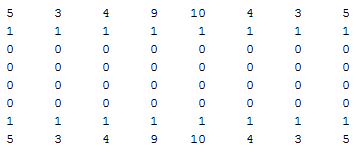
\includegraphics[width=0.6\textwidth]{chessboardmatrix}
\caption{The $chessboard$ matrix at game start}
\label{fig:chess1}
\end{figure}

\begin{figure}[H]
\centering
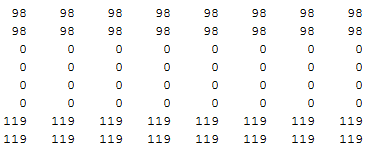
\includegraphics[width=0.62\textwidth]{piece_colour}
\caption{The $piece\_colour$ matrix at game start}
\label{fig:chess2}
\end{figure}

\subsection{Movement files}
\indent\indent Each piece type has its own movement function. This function takes in the position and colour of the piece and the chessboard and generates a matrix that shows all the possible legal moves that piece can make. Empty positions into which the piece can move are denoted by the number 1. Positions currently occupied by the opponent, where the piece can move and make a capture are denoted by the number 2. (See $Fig.$ 4,5)

\begin{figure}[H]
\centering
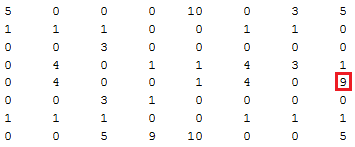
\includegraphics[width=0.6\textwidth]{random_board}
\caption{A random board with the queen highlighted}
\label{fig:chess1}
\end{figure}

\begin{figure}[H]
\centering
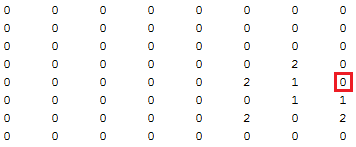
\includegraphics[width=0.6\textwidth]{queen_capture}
\caption{Possible moves of the queen - "1" indicates empty squares, "2" indicates potential captures}
\label{fig:chess1}
\end{figure}

\subsubsection{Pawn Movement}
\begin{figure}[H]
\centering
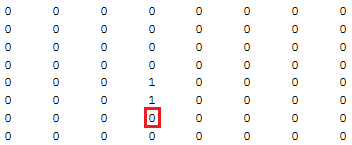
\includegraphics[width=0.6\textwidth]{pawn_movement}
\caption{Possible moves of a pawn from the highlighted square}
\label{fig:chess1}
\end{figure}

\subsubsection{Knight Movement}
\begin{figure}[H]
\centering
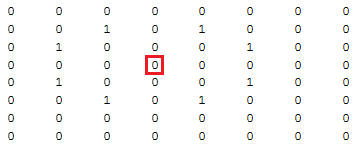
\includegraphics[width=0.6\textwidth]{knight_movement}
\caption{Possible moves of a knight from the highlighted square}
\label{fig:chess1}
\end{figure}

\subsubsection{Bishop Movement}
\begin{figure}[H]
\centering
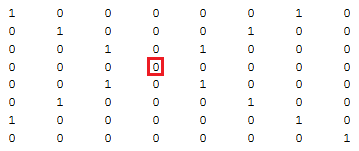
\includegraphics[width=0.6\textwidth]{bishop_movement}
\caption{Possible moves of a bishop from the highlighted square}
\label{fig:chess1}
\end{figure}

\subsubsection{Rook Movement}
\begin{figure}[H]
\centering
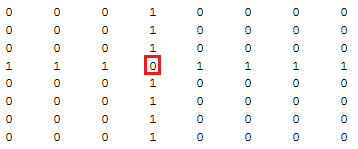
\includegraphics[width=0.6\textwidth]{rook_movement}
\caption{Possible moves of a rook from the highlighted square}
\label{fig:chess1}
\end{figure}

\subsubsection{Queen Movement}
\begin{figure}[H]
\centering
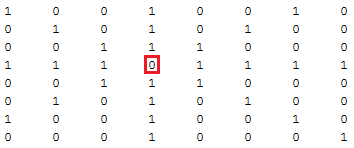
\includegraphics[width=0.6\textwidth]{queen_movement}
\caption{Possible moves of a queen from the highlighted square}
\label{fig:chess1}
\end{figure}

\subsubsection{King Movement}
\begin{figure}[H]
\centering
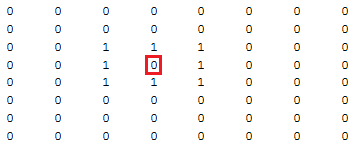
\includegraphics[width=0.6\textwidth]{king_movement}
\caption{Possible moves of a king from the highlighted square}
\label{fig:chess1}
\end{figure}


\subsection{Special moves}
The FOVEROS Chess Engine is programmed to execute special moves such as castling, en passant and pawn promotion. 
However in the case of en passant, the move is not restricted to the first opportunity of its execution.

\subsubsection{Castling}
\begin{figure}[H]
\centering
\begin{subfigure}{0.5\textwidth}
  \centering
  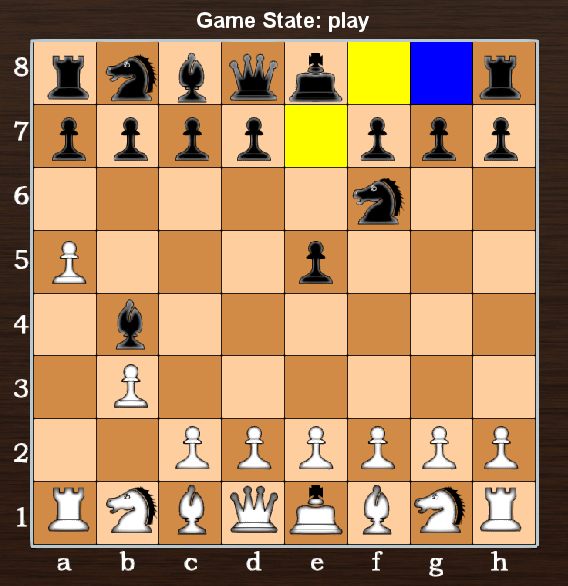
\includegraphics[width=0.9\linewidth]{Castling1}
  \caption{Board shows possiblity of castling}
  \label{fig:sub1}
\end{subfigure}%
\begin{subfigure}{0.5\textwidth}
  \centering
  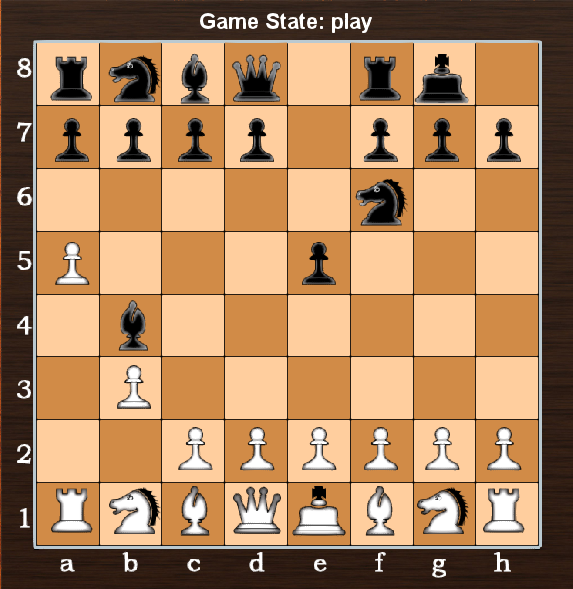
\includegraphics[width=0.9\linewidth]{Castling2}
  \caption{Castling took place}
  \label{fig:sub2}
\end{subfigure}
\caption{Before and after Castling}
\label{fig:test}
\end{figure}

\subsubsection{En passant}
\begin{figure}[H]
\centering
\begin{subfigure}{0.5\textwidth}
  \centering
  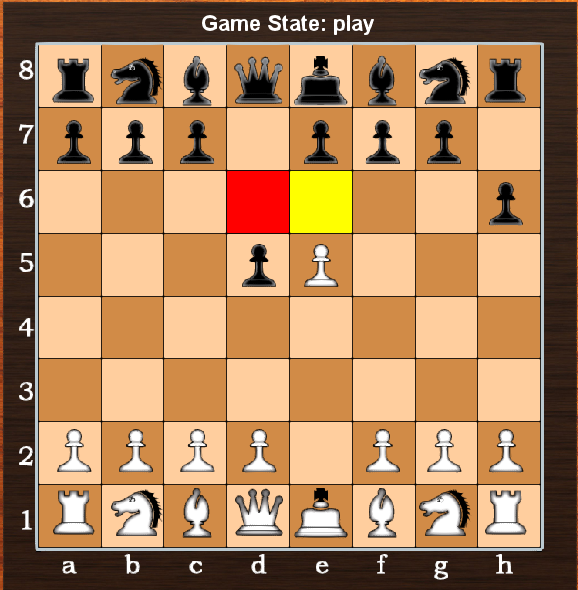
\includegraphics[width=0.91\linewidth]{Enpassant1}
  \caption{Board shows possiblity of En passant}
  \label{fig:sub1}
\end{subfigure}%
\begin{subfigure}{0.5\textwidth}
  \centering
  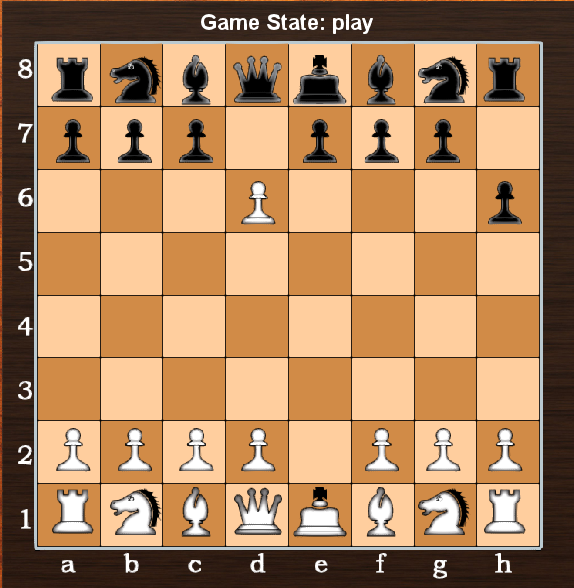
\includegraphics[width=0.9\linewidth]{Enpassant2}
  \caption{En passant took place}
  \label{fig:sub2}
\end{subfigure}
\caption{Before and after En passant}
\label{fig:test}
\end{figure}

\subsubsection{Pawn promotion}
\begin{figure}[H]
\centering
\begin{subfigure}{0.5\textwidth}
  \centering
  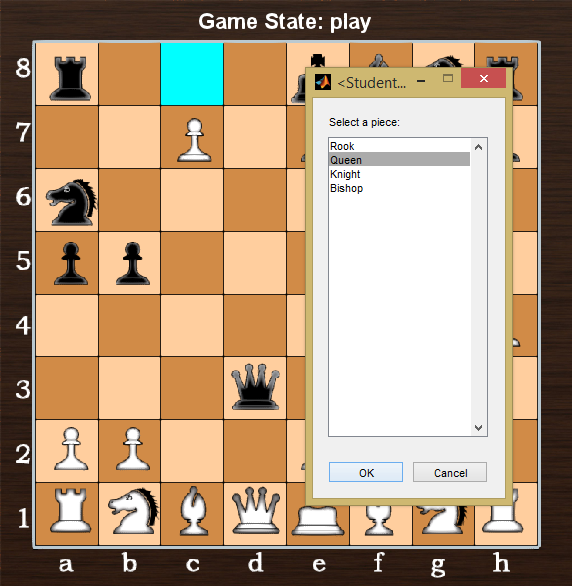
\includegraphics[width=0.91\linewidth]{Pawnpromo1}
  \caption{Board shows possiblity of Pawn promotion}
  \label{fig:sub1}
\end{subfigure}%
\begin{subfigure}{0.5\textwidth}
  \centering
  \includegraphics[width=0.9\linewidth]{Pawnpromo2}
  \caption{Pawn promotion took place}
  \label{fig:sub2}
\end{subfigure}
\caption{Before and after Pawn promotion}
\label{fig:test}
\end{figure}

\subsection{Board Analysis}
\subsubsection{Analyseboard Function}
The function $analyseboard$ looks at all the pieces of a specified colour and determines where every piece is able to move. This function generates the matrix $potentialmoves$ containing all the possible moves that side can make and a vector $capt\_index$ containing the locations of possible captures. 
This function lends itself to the $KingCheck$ and $checkmate$ functions.

\subsubsection{KingCheck Function}
The function $KingCheck$ uses the results of $analyseboard$ to determine if the king is in check. The king is in check when its position overlaps with the opponent’s potential moves. This function lends itself to the $checkmate$ function.

\subsubsection{Checkmate Function}
The function $checkmate$ determines if the current board is a checkmate state for the specified colour. This function generates all the possible moves searching for any legal moves that can be made. Even if one legal move exists, then the board is determined to not be in a state of checkmate.
\newline
$checkmate$ assumes that the king is already in check and hence must always be paired with the $KingCheck$ function.


\newpage
\section{Front-end}

\subsection{Click Series of Functions}

This section discusses the following functions: 
\begin{itemize}
\item $ClickPiece$
\item $ClickCapturePiece$
\item $ClickMovePiece$
\item $ClickPawnPromo$
\item $ClickCastling$
\item $ClickEnPassant$
\end{itemize}


The purpose of the click series of functions is to enable the user to make selections on the GUI that translate into a new board state.  $ClickPiece$ is embedded in the ButtonDown function of the images on the plot. When a user selects a piece, it’s moves are highlighted as shown. In essence, $ClickPiece$ acts like a switch to embed the other 5 functions into the right squares so that the user is able to make the corresponding move.(See $Fig.$ 15)
\\*\\
Line 9 – 17: Determines the colour that is at play.
\\*\\
Line 19 - 31: Determines the coordinates of the user selection and makes the relevant coordinate conversions for the backend.
\\*\\
Line 34 – 51: Determines the piece that is selected and generates its possible moves.
\\*\\
Line 52 – 104: The squares of the board are redrawn with colours corresponding to the matrix of the possiblemoves. For example: A capture is shown in the possible moves matrix as ‘2’ and the corresponding square is coloured red.
\\*\\
Lines 108 – 134: This section redraws the pieces on the board and embeds “ClickPiece” again so that the user can reselect another piece if necessary.\newline

\begin{figure}[H]
\centering
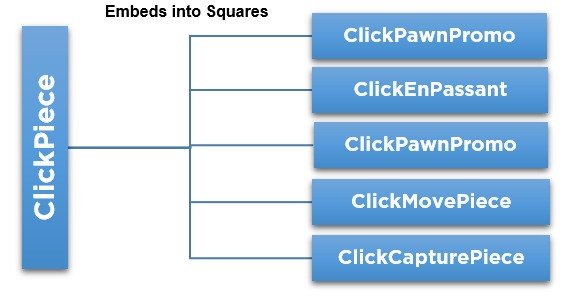
\includegraphics[width=0.7\textwidth]{flow_chart}
\caption{Flow chart showing the activation of $ClickPiece$}
\label{fig:chess1}
\end{figure}

This section will detail the code of the 5 click functions for $ClickMovePiece$, $ClickCapturePiece$, $ClickCastling$, $ClickEnPassant$ and $ClickPawnPromo$. The code for all of them are very similar, except their function specific parts. The code explanation below details the $ClickMovePiece$ function:
\\*\\
Line 8 – 14 : Determines the colour at play
\\*\\
Line 17 – 32: Determines the coordinates that player has chosen to move the piece and makes the relevant coordinate conversions for the backend.
\\*\\
Line 40 – 60: The move is done on a future board state to validate that the King will not left in check as a result of the move which constitutes and illegal move. This is where the different click functions will have function specific coordinate transformations to facilitate their purpose.
\\*\\
Line 73 – 75: If the move is valid, the future board state is saved as the accepted board state.
\\*\\
Line 77 – 94: Validates if the opposing King is in check as a result of the move and also validates of checkmate or stalemate have taken place.
\\*\\
Line 99 – 128: The board is redrawn to reflect the new board state.
\\*\\
Line 131 – 138: Based on the user’s player choice, the next move is passed to the relevant control function.


\subsection{Graphical User Interface}
The GUI is designed to show the relevant board stats and game messages. The user is able to select from different settings for the GUI. It also plots the scores on the graph to show the progression of both players with each turn.
\begin{figure}[H]
\centering
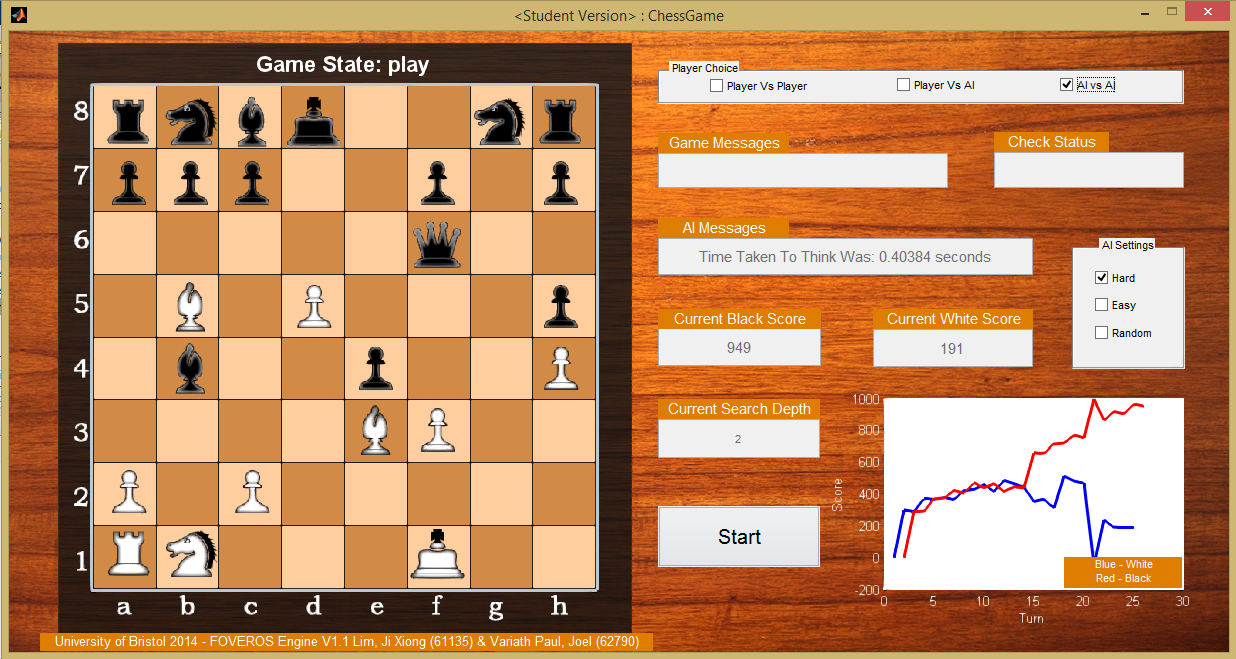
\includegraphics[width=1\textwidth]{GUI}
\caption{FOVEROS Chess Engine GUI}
\label{fig:chess1}
\end{figure}

\newpage
\section{Artificial Intelligence}

\subsection{Brute Force Approach}
\indent\indent The approach to implementing computer thought is through brute force calculations. The strength in computer systems lies in its ability to perform a large amounts of computation in a short period of time. Therefore, it has the ability to generate all future board states up to a certain depth. Depth is the number of turns ahead of the current board state that is generated. 

\subsubsection{Minimax Algorithm}
\indent\indent The generation of board states must be aided by an algorithm to evaluate and save the best board states. This is an adversarial search problem where only 2 players are competing. In order to make the optimal decision for a certain player, the MiniMax strategy is used. The idea is that from a certain player’s perspective, the objective is to maximise the player’s advantage and to minimise the opponent’s advantage. The generation starts from the “Initial State” and branches out until it reaches the “Leaf Nodes” or “Terminal Nodes” where the board is evaluated and the results backed up the tree as the recursion unwinds.\cite{chess1}
\\*\\
\indent Generation of board states however is a computationally expensive task especially to deeper depths. The branching factor can be defined as the number of children per node. The average branching factor for chess positions is 35 to 38 moves per position.  Therefore, 38\textsuperscript{2} (1,444) game states need to be evaluated at depth 2, 38\textsuperscript{3} (54,872) game states need to be evaluated at depth 3, 38\textsuperscript{4} (2,085,136) game states need to be evaluated at depth 4. It is clear that the number of game states will continue to grow at an exponential rate.\cite{chess2}

\subsubsection{Alpha-Beta Pruning}
\indent\indent An algorithm that “prunes” the search tree needs to use to eliminate parts of the tree that will have no effect on the final result of the tree. Alpha Beta pruning is a method to prune the search tree. Alpha is the maximum lower bound of the possible solutions and Beta is the minimum upper bound of the possible solutions. The search proceeds down to the first terminal node of the tree, the board score is backed up the tree and becomes either the alpha or beta value of the node above it depending on whether it is a minimum or maximum player. 

\begin{figure}[H]
\centering
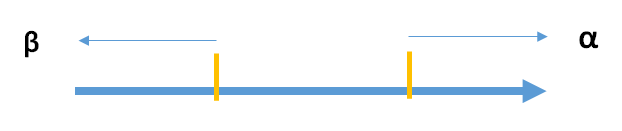
\includegraphics[width=0.7\textwidth]{alphabeta}
\caption{Figure shows $\alpha$-$\beta$ pruning criteria}
\label{fig:chess1}
\end{figure}

\indent The search then proceeds and references back to the alpha and beta value before it. If the values are found to be lower than the maximum lower bound or higher than the minimum upper bound, the values of alpha and beta are reassigned to the new values. However, pruning occurs when alpha is greater than beta and the branches leading from the selected node are not evaluated because it will not change the overall result of the tree. It will not change it because there is no overlap between the maximum lower bound and the minimum upper bound as shown in the figure.\cite{chess3}
\\*\\
\indent By implementing Alpha Beta pruning with random move ordering, the average number of nodes to be evaluated will be dropped to $b^{3d/4}$ from $b^d$. This means that Alpha Beta pruning is able to perform a depth 4 calculation at roughly the same speed as a depth 3 without Alpha Beta pruning.\cite{chess4}

\subsection{Generation of Moves}
\indent\indent The function $AI\_GenerateAllMoves$ generates all nodes up to a certain depth, implements the MiniMax Algorithm and Alpha Beta pruning. The function does this via the recursion method where the function calls itself within its function. This is useful because in the MiniMax algorithm we require the values to be backed up the tree and recursion does that inherently.
\\*\\
Line 1 – 15: Determines the colour at play
\\*\\
Line 20 – 26: At Terminal Node, the board is evaluated
\\*\\
Line 29 – 122: Implementation for the Maximum Player
\\*\\
Line 126 – 222: Implementation for the Minimum Player\newline
\\*\\
\indent The implementation for the Maximum and Minimum player are the same but with slightly different parameters. The general structure is discussed below for the Maximum Player.
\\*\\
Line 33 – 36: The coordinates of the current colour pieces are found. The arrangement of the pieces in the vector is randomly permutated.
\\*\\
Line 42 – 57: For each of the pieces, the individual possible moves are generated
\\*\\
Line 63 – 67: The coordinates of the possible moves are randomly permutated
\\*\\
Line 70 – 87: The potential future board state is generated.
\\*\\
Line 89 – 116: The board is evaluated for legality, if found to be illegal it will be ignored. If it is valid, the function calls itself again. The parameters passed are the new node and the depth is decreased. The alpha-beta pruning condition is also implemented here.

\subsection{Heuristic Analysis}
\indent\indent The function $heuristicanalysis$ examines the board from a given player’s point of view. The goal of this function is to assign a numerical value(boardscore) to each board depending on a given set of conditions. These conditions determine if a move is good or bad.\cite{chess6}\cite{chess7}

\noindent A move is judged to be good:
\begin{itemize}
\item If it opens up possibilities to capture opponent’s pieces
\item If it increases the number of pieces captured
\item If it opens up space for other pieces to move
\item If it increases control of the centre of the board
\item If it enables the king to castle
\item If it brings the pawns closer to the end of the board for promotion
\item If it leads to checks and checkmates on the opponent
\end{itemize}

\noindent A move is judged to be bad:
\begin{itemize}
\item If it causes threats to its own pieces
\item If it decreases the number of its own pieces
\item If it leads to the opponent’s pawns being promoted
\item If it leads to its own king being checked or checkmated
\end{itemize}

Each of these conditions is assigned a specific $gainfactor$. The more important the condition is, the higher the numerical value of the $gainfactor$. Good moves have positive $gainfactor$ which encourage the AI to make those moves, while bad moves have negative $gainfactor$, discouraging the AI.
\newline
For example, a move that leads to the opponent king being checkmated is assigned the highest possible score of 99999, while a move that leads to its own checkmate is assigned the lowest possible score of -99999.

The values of the Gain factors depend on the level of difficulty the player has chosen. In a ‘Random’ game the gains are all set to 0 and have no influence on the moves. In an ‘Easy’ game, the gains are such that it’s easy for the player to make threats and capture pieces. In a ‘Hard’ game, the gains ensure that the AI plays aggressively. 


\subsection{AI Control}
\indent\indent The function $AIControl$ sets the depth parameters for $AI\_GenerateAllMoves$, plots the board scores as seen on the GUI and validates check/checkmate/stalemate for both colours.


\newpage
\section{Results}
\begin{figure}[H]
\centering
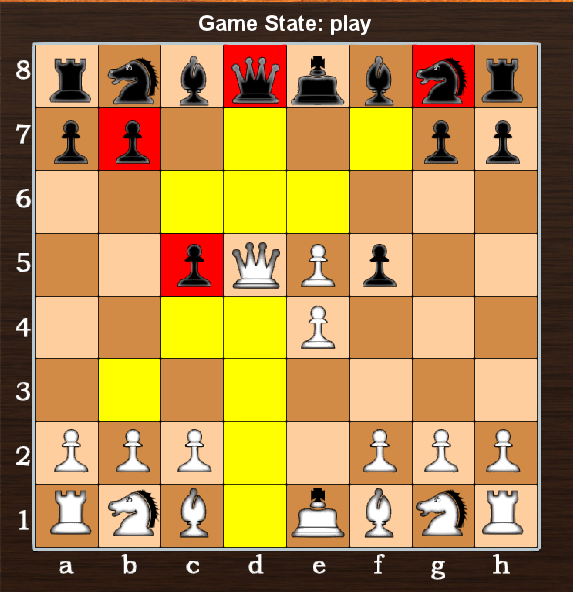
\includegraphics[width=0.6\textwidth]{Queen}
\caption{Possible moves of Queen in game}
\label{fig:chess1}
\end{figure}

\begin{figure}[H]
\centering
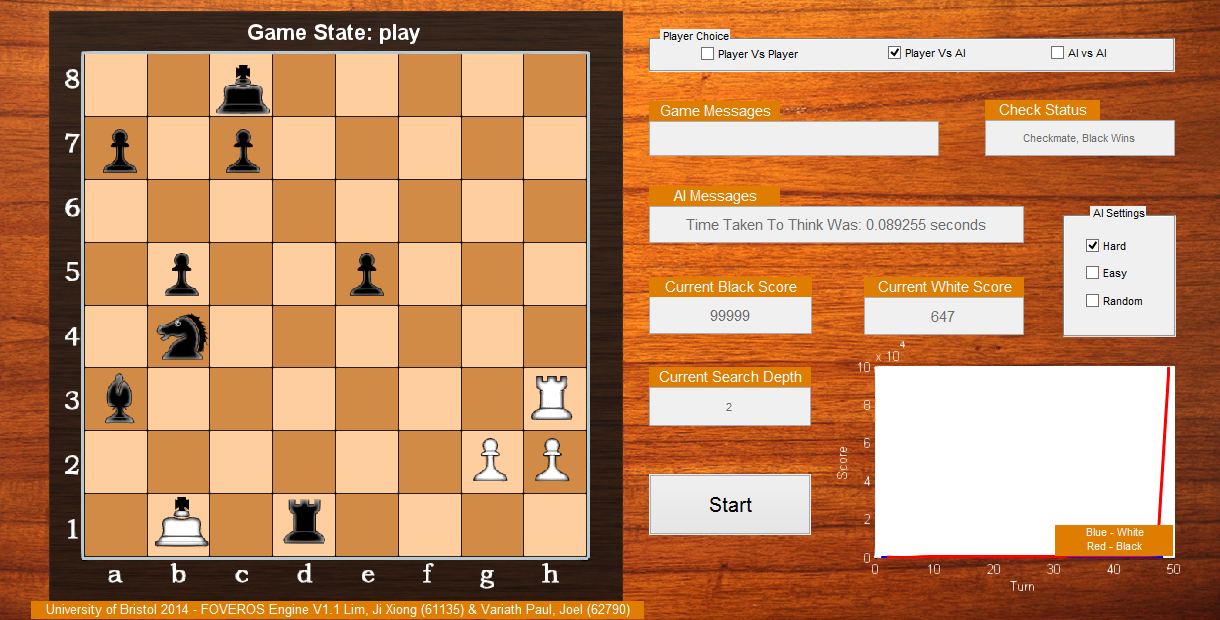
\includegraphics[width=1\textwidth]{black_checkmate}
\caption{Checkmate by Black}
\label{fig:chess1}
\end{figure}

\begin{figure}[H]
\centering
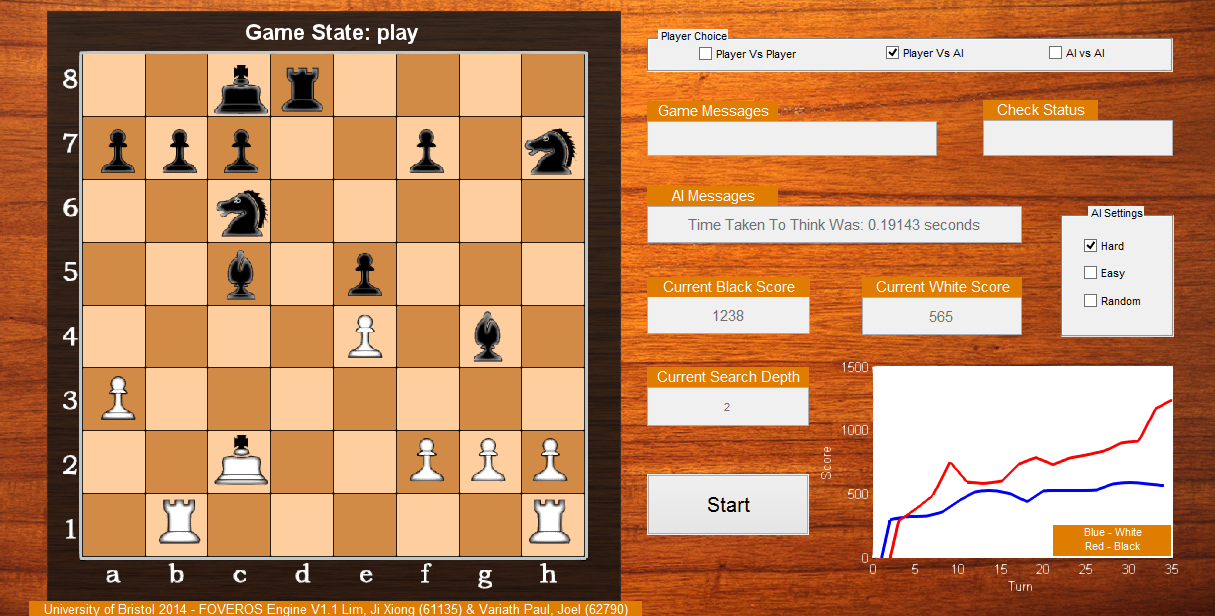
\includegraphics[width=1\textwidth]{AI_castling}
\caption{AI has Castled}
\label{fig:chess1}
\end{figure}

\begin{table}[h]
\centering
\begin{tabular}{|l|l|l|l|l|l|l|}
\hline
\multirow{2}{*}{Depth} & \multicolumn{2}{l|}{\begin{tabular}[c]{@{}l@{}}Without Alpha\\   Beta Pruning\end{tabular}} & \multicolumn{2}{l|}{\begin{tabular}[c]{@{}l@{}}With Alpha\\   Beta Pruning\end{tabular}} & \multicolumn{2}{l|}{\begin{tabular}[c]{@{}l@{}}Percentage Reduction Between\\   With and Without Pruning\end{tabular}} \\ \cline{2-7} 
                       & Time/s                                      & Nodes                               & Time/s                                 & Nodes                                 & Time                                 & Node                                \\ \hline
1                      & 0.046                                       & 20                                            & 0.05                                   & 20                                              & 8.70                          & 0                                   \\ \hline
2                      & 1.45                                        & 620                                           & 0.31                                   & 136                                             & -78.6                         & -78.1                        \\ \hline
3                      & 46.7                                        & 13928                                         & 1.98                                   & 832                                             & -95.8                         & -94.0                         \\ \hline
4                      & 1365                                        & 420180                                        & 23.4                                   & 8535                                            & -98.3                        & -98.0                        \\ \hline
5                      & \textgreater2400                            & \textgreater720000                            & 96                                     & 33022                                           &  -                                    &     -                                \\ \hline
\end{tabular}
\caption{Performance results of $\alpha$-$\beta$ pruning}
\label{fig:chess1}
\end{table}


\newpage
\section{Discussions}

\subsection{Tuning}
\indent\indent Tuning is the process of finding the optimum gains for the different scores in the Heuristics Analysis function. The different gains increase or decrease the effect of different parameters on the board score. Tuning is a difficult process because the values are relative and therefore trial and error is to be used to determine the optimum value. By comparison, the programmers of the legendary Deep Blue machine had made plausible initial guesses for values and there was a lot of uncertainty to what the correct values should be.\cite{chess5}

	The first objective for optimum tuning was to reach a high level of aggressiveness for the AI as that is most noticeable feature. This would be demonstrated by making captures when the opportunity presents itself.  The second objective was to prevent moves that would jeopardise its own pieces and that also includes encouraging castling to shield the King. The third objective was to increase likelihood of check and checkmate.

	The current gains that are set are based on trial and error. Based on the results, some of the features have demonstrated itself rather obviously. $Fig.$ 19 shows the situation of Player Vs AI and the AI has successfully checkmated the player in a rather creative arrangement that involves 3 different pieces. The graph also shows that the boardscore has been maximised for that colour which is the correct output from the Heuristics Analysis.

	$Fig.$ 20 also shows the AI using Castling it its advantage in the late game by allowing the rook to come out and the King to seek shelter behind the pawns thus increasing its boardscore as a result of the move. 

	A deficiency that is quite common in the AI was that the AI tended to make captures that would lead to its own piece being captured. The pay off would sometimes be less than the value of the piece being sacrificed. The AI would also pass off captures sometimes but it is rare.

\subsection{Alpha Beta Pruning Efficiency}
\indent\indent $Table$ 1 shows the various timings and number of nodes at a certain depth. The results is as expected, the number of nodes that need to be evaluated at a certain depth have an exponential relationship with the depth itself. The Alpha Beta Pruning implementation cuts down the time taken by a very substantial amount. This is also as expected as discussed in the Artificial Intelligence section. It should enable the system to go 1 depth deeper with Alpha Beta Pruning at the same speed as without the Alpha Beta Pruning.


\newpage
\section{Conclusions}

\indent\indent The FOVEROS Engine which means “Awesome” in Greek employs basic understanding of the tree search algorithm, MiniMax Theory, Alpha Beta pruning optimisation. It has also met the design aim of being a functional chessboard that has inbuilt rules and able to execute all the special moves without problems.

	There are further improvements that can be made for this engine. The first is the integration of a database of opening moves. This will enable the engine to have greater flexibility in its opening moves and open up more possibilities for the engine. This can be done by setting the AI to respond with predefined moves for the first 3 rounds based on the response of the opponent.

	Further optimisations to the tree-search algorithm can be looked into. The first is Iterative Deepening which encourages deeper searches until the pre-allocated time is exhausted. It is a time management strategy in depth-first searches and has benefits for move ordering and pruning.\cite{chess9}

	FOVEROS employs random move ordering in the algorithm and so dynamic move ordering techniques should be looked into. The benefits of Alpha Beta pruning are only tangible if the best move is presented as soon as possible so that pruning can take place immediately.\cite{chess8}
 


\newpage
\bibliographystyle{plain}
\bibliography{ChessReport}
\newpage

\appendix
\section{Appendix: The Code}
\subsection{Back-end}
\subsubsection{MovementRook.m}
\begin{lstlisting}

function [possiblemoves] = MovementRook(chessboard,piece_colour,p_x,p_y)

%Initialisation values --------------------------------------------------
r_colour = piece_colour(p_x,p_y);
possiblemoves = zeros(8,8);

%This section allows movement in vertical direction -----------------------
i = 1;
while(p_x+i<9)
    if(piece_colour(p_x+i,p_y)== r_colour)
        break
    end
    if(piece_colour(p_x+i,p_y)~= r_colour && chessboard(p_x+i,p_y)~=0)
        possiblemoves(p_x+i,p_y) = 2;
        break
    end
    possiblemoves(p_x+i,p_y) = 1;
    i = i+1;
end
            
i = 1;
while(p_x-i>0)
    if(piece_colour(p_x-i,p_y)== r_colour)
        break
    end
     if(piece_colour(p_x-i,p_y)~= r_colour && chessboard(p_x-i,p_y)~=0)
        possiblemoves(p_x-i,p_y) = 2;
        break
    end
    possiblemoves(p_x-i,p_y) = 1;
    i = i+1;
end

%This section allows movement in the horizontal direction
i = 1;
while(p_y+i<9)
    if(piece_colour(p_x,p_y+i)== r_colour)
        break
    end
    if(piece_colour(p_x,p_y+i)~= r_colour && chessboard(p_x,p_y+i)~=0)
        possiblemoves(p_x,p_y+i) = 2;
        break
    end
    possiblemoves(p_x,p_y+i) = 1;
    i = i+1;
end

i = 1;
while(p_y-i>0)
    if(piece_colour(p_x,p_y-i)== r_colour)
        break
    end
    if(piece_colour(p_x,p_y-i)~= r_colour && chessboard(p_x,p_y-i)~=0)
        possiblemoves(p_x,p_y-i) = 2;
        break
    end
    possiblemoves(p_x,p_y-i) = 1;
    i = i+1;
end

%-------------------------------------------------------------------------

end
\end{lstlisting}

\subsubsection{MovementQueen.m}
\begin{lstlisting}
function [possiblemoves] = MovementQueen(chessboard,piece_colour,p_x,p_y)

%Initialisation values --------------------------------------------------
possiblemoves = zeros(8,8);
r_colour = piece_colour(p_x,p_y);

%This section allows movement in / direction -----------------------------
i=1;
while(p_x+i<9 && p_y+i<9)
    if(piece_colour(p_x+i,p_y+i)== r_colour)
        break
    end
    if(piece_colour(p_x+i,p_y+i)~= r_colour && chessboard(p_x+i,p_y+i)~=0)
        possiblemoves(p_x+i,p_y+i) = 2;
        break
    end
    possiblemoves(p_x+i,p_y+i) = 1;
    i = i+1;
end

i=1;
while(p_x-i>0 && p_y-i>0)
    if(piece_colour(p_x-i,p_y-i)== r_colour)
        break
    end
    if(piece_colour(p_x-i,p_y-i)~= r_colour && chessboard(p_x-i,p_y-i)~=0)
        possiblemoves(p_x-i,p_y-i) = 2;
        break
    end
    possiblemoves(p_x-i,p_y-i) = 1;
    i = i+1;
end

%This section allows movement in the \ direction-------------------------
i=1;
while(p_x+i<9 && p_y-i>0)
    if(piece_colour(p_x+i,p_y-i)== r_colour)
        break
    end
    if(piece_colour(p_x+i,p_y-i)~= r_colour && chessboard(p_x+i,p_y-i)~=0)
        possiblemoves(p_x+i,p_y-i) = 2;
        break
    end
    possiblemoves(p_x+i,p_y-i) = 1;
    i = i+1;
end

i=1;
while(p_x-i>0 && p_y+i<9)
    if(piece_colour(p_x-i,p_y+i)== r_colour)
        break
    end
    if(piece_colour(p_x-i,p_y+i)~= r_colour && chessboard(p_x-i,p_y+i)~=0)
        possiblemoves(p_x-i,p_y+i) = 2;
        break
    end
    possiblemoves(p_x-i,p_y+i) = 1;
    i = i+1;
end

%This section allows movement in vertical direction -----------------------------
i = 1;
while(p_x+i<9)
    if(piece_colour(p_x+i,p_y)== r_colour)
        break
    end
    if(piece_colour(p_x+i,p_y)~= r_colour && chessboard(p_x+i,p_y)~=0)
        possiblemoves(p_x+i,p_y) = 2;
        break
    end
    possiblemoves(p_x+i,p_y) = 1;
    i = i+1;
end
            
i = 1;
while(p_x-i>0)
    if(piece_colour(p_x-i,p_y)== r_colour)
        break
    end
     if(piece_colour(p_x-i,p_y)~= r_colour && chessboard(p_x-i,p_y)~=0)
        possiblemoves(p_x-i,p_y) = 2;
        break
    end
    possiblemoves(p_x-i,p_y) = 1;
    i = i+1;
end

%This section allows movement in the horizontal direction-------------------------
i = 1;
while(p_y+i<9)
    if(piece_colour(p_x,p_y+i)== r_colour)
        break
    end
    if(piece_colour(p_x,p_y+i)~= r_colour && chessboard(p_x,p_y+i)~=0)
        possiblemoves(p_x,p_y+i) = 2;
        break
    end
    possiblemoves(p_x,p_y+i) = 1;
    i = i+1;
end

i = 1;
while(p_y-i>0)
    if(piece_colour(p_x,p_y-i)== r_colour)
        break
    end
    if(piece_colour(p_x,p_y-i)~= r_colour && chessboard(p_x,p_y-i)~=0)
        possiblemoves(p_x,p_y-i) = 2;
        break
    end
    possiblemoves(p_x,p_y-i) = 1;
    i = i+1;
end
%-------------------------------------------------------------------------

end
\end{lstlisting}

\subsubsection{MovementPawn.m}
\begin{lstlisting}
function [possiblemoves] = MovementPawn(chessboard,piece_colour,num_moves,p_x,p_y)

%Initialisation values --------------------------------------------------
r_colour = piece_colour(p_x,p_y);
possiblemoves = zeros(8,8);

%This section allows all movements after checking whether it exceeds the board or not ---------------
switch r_colour
    case 119 %White case
        %En passant-------------------------------------------------------
        if (p_x==4)
            
            if(p_x-1>0 && p_y-1 >0) %Capture left
                if(piece_colour(p_x,p_y-1)~=r_colour && chessboard(p_x,p_y-1)==1 && num_moves(p_x,p_y-1)==1)
                    possiblemoves(p_x-1,p_y-1) = 3;
                end
            end

            if(p_x-1>0 && p_y+1<9) %Capture right
                if(piece_colour(p_x,p_y+1)~=r_colour && chessboard(p_x,p_y+1)==1 && num_moves(p_x,p_y+1)==1)
                    possiblemoves(p_x-1,p_y+1) = 3;
                end    
            end
        
        end
        
        if(p_x-1>0) %Forward movement
            if(chessboard(p_x-1,p_y)==0)
                possiblemoves(p_x-1,p_y) = 1;
            end
        end
        
        %Initial forward movement
        if(p_x==7 && chessboard(p_x-2,p_y)==0 && chessboard(p_x-1,p_y)==0)
        possiblemoves(p_x-2,p_y) = 1;
        end

        if(p_x-1>0 && p_y-1 >0) %Capture left
            if(piece_colour(p_x-1,p_y-1)~=r_colour && chessboard(p_x-1,p_y-1)~=0)
                possiblemoves(p_x-1,p_y-1) = 2;
                   if(p_x==2) %Capture and pawn promotion
                      possiblemoves(p_x-1,p_y-1) = 5;
                   end
            end
        end

        if(p_x-1>0 && p_y+1<9) %Capture right
            if(piece_colour(p_x-1,p_y+1)~=r_colour && chessboard(p_x-1,p_y+1)~=0)
                possiblemoves(p_x-1,p_y+1) = 2;
                   if(p_x==2) %Capture and pawn promotion
                      possiblemoves(p_x-1,p_y+1) = 5;
                   end
            end
        end    
        
        %Pawn promotion----------------------------------------------------
        if(p_x==2) 
            if(chessboard(p_x-1,p_y)==0)
                possiblemoves(p_x-1,p_y) = 5;
            end
        end
       
    case 98 %Black Case
    
        %En passant-------------------------------------------------------
        if (p_x==5)
            
            if(p_x-1>0 && p_y-1 >0) %Capture left
                if(piece_colour(p_x,p_y-1)~=r_colour && chessboard(p_x,p_y-1)==1 && num_moves(p_x,p_y-1)==1)
                    possiblemoves(p_x+1,p_y-1) = 3;
                end
            end

            if(p_x-1>0 && p_y+1<9) %Capture right
                if(piece_colour(p_x,p_y+1)~=r_colour && chessboard(p_x,p_y+1)==1 && num_moves(p_x,p_y+1)==1)
                    possiblemoves(p_x+1,p_y+1) = 3;
                end    
            end
        
        end
        
        if(p_x+1<9) %Forward movement
            if(chessboard(p_x+1,p_y)==0) 
                possiblemoves(p_x+1,p_y) = 1;
            end
        end

        %Initial Forward movement
        if(p_x==2 && chessboard(p_x+2,p_y)==0 && chessboard(p_x+1,p_y)==0)
            possiblemoves(p_x+2,p_y) = 1;
        end
        
        if(p_x+1<9 && p_y-1>0) %Capture left
            if(piece_colour(p_x+1,p_y-1)~=r_colour && chessboard(p_x+1,p_y-1)~=0)
                possiblemoves(p_x+1,p_y-1) = 2;
                  if(p_x==7) %Capture and pawn promotion
                      possiblemoves(p_x+1,p_y-1) = 5;
                   end
            end
        end
        
        if(p_x+1<9 && p_y+1<9) %Capture right
            if(piece_colour(p_x+1,p_y+1)~=r_colour && chessboard(p_x+1,p_y+1)~=0)
                possiblemoves(p_x+1,p_y+1) = 2;
                   if(p_x==7) %Capture and pawn promotion
                      possiblemoves(p_x+1,p_y+1) = 5;
                   end
            end   
        end
        
        %Pawn promotion----------------------------------------------------
        if(p_x==7)
            if(chessboard(p_x+1,p_y)==0) 
                possiblemoves(p_x+1,p_y) = 5;
            end
        end
   
end
%-------------------------------------------------------------------------
end
\end{lstlisting}

\subsubsection{MovementKnight.m}
\begin{lstlisting}
function [possiblemoves] = MovementKnight(chessboard,piece_colour,p_x,p_y)

%Initialisation values --------------------------------------------------
r_colour = piece_colour(p_x,p_y);
possiblemoves = zeros(8,8);

%This sections allows L shaped movements for knight
if(p_x-2>0 & p_y-1>0)
    if (piece_colour(p_x-2,p_y-1)~= r_colour && chessboard(p_x-2,p_y-1)~=0)
        possiblemoves(p_x-2,p_y-1) = 2;
    elseif (piece_colour(p_x-2,p_y-1)== r_colour)
        ;
    else
        possiblemoves(p_x-2,p_y-1) = 1;
    end
end

if(p_x-2>0 & p_y+1<9)
    if (piece_colour(p_x-2,p_y+1)~= r_colour && chessboard(p_x-2,p_y+1)~=0)
        possiblemoves(p_x-2,p_y+1) = 2;
    elseif (piece_colour(p_x-2,p_y+1)== r_colour)
        ;
    else
        possiblemoves(p_x-2,p_y+1) = 1;
    end
end

if(p_x-1>0 & p_y-2>0)
    if (piece_colour(p_x-1,p_y-2)~= r_colour && chessboard(p_x-1,p_y-2)~=0)
        possiblemoves(p_x-1,p_y-2) = 2;
    elseif (piece_colour(p_x-1,p_y-2)== r_colour)
        ;
    else
        possiblemoves(p_x-1,p_y-2) = 1;
    end
end

if(p_x-1>0 & p_y+2<9)
    if (piece_colour(p_x-1,p_y+2)~= r_colour && chessboard(p_x-1,p_y+2)~=0)
        possiblemoves(p_x-1,p_y+2) = 2;
    elseif (piece_colour(p_x-1,p_y+2)== r_colour)
        ;
    else
        possiblemoves(p_x-1,p_y+2) = 1;
    end
end

if(p_x+1<9 & p_y-2>0)
    if (piece_colour(p_x+1,p_y-2)~= r_colour && chessboard(p_x+1,p_y-2)~=0)
        possiblemoves(p_x+1,p_y-2) = 2;
    elseif (piece_colour(p_x+1,p_y-2)== r_colour)
        ;
    else
        possiblemoves(p_x+1,p_y-2) = 1;
    end
end

if(p_x+1<9 & p_y+2<9)
    if (piece_colour(p_x+1,p_y+2)~= r_colour && chessboard(p_x+1,p_y+2)~=0)
        possiblemoves(p_x+1,p_y+2) = 2;
    elseif (piece_colour(p_x+1,p_y+2)== r_colour)
        ;
    else
        possiblemoves(p_x+1,p_y+2) = 1;
    end
end

if(p_x+2<9 & p_y-1>0)
    if (piece_colour(p_x+2,p_y-1)~= r_colour && chessboard(p_x+2,p_y-1)~=0)
        possiblemoves(p_x+2,p_y-1) = 2;
    elseif (piece_colour(p_x+2,p_y-1)== r_colour)
        ;
    else
        possiblemoves(p_x+2,p_y-1) = 1;
    end
end

if(p_x+2<9 & p_y+1<9)
    if (piece_colour(p_x+2,p_y+1)~= r_colour && chessboard(p_x+2,p_y+1)~=0)
        possiblemoves(p_x+2,p_y+1) = 2;
    elseif (piece_colour(p_x+2,p_y+1)== r_colour)
        ;
    else
        possiblemoves(p_x+2,p_y+1) = 1;
    end
end

%-------------------------------------------------------------------------

end
\end{lstlisting}


\subsubsection{MovementKing.m}
\begin{lstlisting}
function [possiblemoves] = MovementKing(chessboard,piece_colour,num_moves,potential_moves,p_x,p_y)

%Initialisation values --------------------------------------------------
r_colour = piece_colour(p_x,p_y);
possiblemoves = zeros(8,8);

%This section allows all movements after checking whether it exceeds the board or not 
%and ensures that the king is not moving into square that is in check ---------------

%------------------------------------------------------------------------
%                        Movement (8 Directions)
%------------------------------------------------------------------------

    
    if(p_x+1<9)
        if (piece_colour(p_x+1,p_y)~= r_colour && chessboard(p_x+1,p_y)~=0)
            possiblemoves(p_x+1,p_y) = 2;
        elseif (piece_colour(p_x+1,p_y)== r_colour)
            ;
        else
            possiblemoves(p_x+1,p_y) = 1;
        end
    end
    
    
    if(p_x+1<9 && p_y+1<9)
        if (piece_colour(p_x+1,p_y+1)~= r_colour && chessboard(p_x+1,p_y+1)~=0)
            possiblemoves(p_x+1,p_y+1) = 2;
        elseif (piece_colour(p_x+1,p_y+1)== r_colour)
            ;
        else
            possiblemoves(p_x+1,p_y+1) = 1;
        end
    end
    
    
    if(p_x+1<9 && p_y-1>0)
        if (piece_colour(p_x+1,p_y-1)~= r_colour && chessboard(p_x+1,p_y-1)~=0)
            possiblemoves(p_x+1,p_y-1) = 2;
        elseif (piece_colour(p_x+1,p_y-1)== r_colour)
            ;
        else
            possiblemoves(p_x+1,p_y-1) = 1;
        end
    end
    
    
    if(p_y+1<9)
        if (piece_colour(p_x,p_y+1)~= r_colour && chessboard(p_x,p_y+1)~=0)
            possiblemoves(p_x,p_y+1) = 2;
        elseif (piece_colour(p_x,p_y+1)== r_colour)
            ;
        else
            possiblemoves(p_x,p_y+1) = 1;
        end
    end
    
    
    if(p_y-1>0)
        if (piece_colour(p_x,p_y-1)~= r_colour && chessboard(p_x,p_y-1)~=0)
            possiblemoves(p_x,p_y-1) = 2;
        elseif (piece_colour(p_x,p_y-1)== r_colour)
            ;
        else
            possiblemoves(p_x,p_y-1) = 1;
        end
    end
    
    
    if(p_x-1>0)
        if (piece_colour(p_x-1,p_y)~= r_colour && chessboard(p_x-1,p_y)~=0)
            possiblemoves(p_x-1,p_y) = 2;
        elseif (piece_colour(p_x-1,p_y)== r_colour)
            ;
        else
            possiblemoves(p_x-1,p_y) = 1;
        end
    end
    
    
    if(p_x-1>0 && p_y+1<9)
        if (piece_colour(p_x-1,p_y+1)~= r_colour && chessboard(p_x-1,p_y+1)~=0)
            possiblemoves(p_x-1,p_y+1) = 2;
        elseif (piece_colour(p_x-1,p_y+1)== r_colour)
            ;
        else
            possiblemoves(p_x-1,p_y+1) = 1;
        end
    end
    
    
    if(p_x-1>0 && p_y-1>0)
        if (piece_colour(p_x-1,p_y-1)~= r_colour && chessboard(p_x-1,p_y-1)~=0)
            possiblemoves(p_x-1,p_y-1) = 2;
        elseif (piece_colour(p_x-1,p_y-1)== r_colour)
            ;
        else
            possiblemoves(p_x-1,p_y-1) = 1;
        end
    end

%-------------------------------------------------------------------------   
%                                  Castling 
%-------------------------------------------------------------------------


%---------------------------- For white king ----------------------------
   
possiblemoves(p_x,p_y)=0;
%-------------------------------------------------------------------------
end
\end{lstlisting}

\subsubsection{MovementBishop.m}
\begin{lstlisting}
function [possiblemoves] = MovementBishop(chessboard,piece_colour,p_x,p_y)

%Initialisation values --------------------------------------------------
r_colour = piece_colour(p_x,p_y);
possiblemoves = zeros(8,8);

%This section allows movement in / direction -----------------------------
i=1;
while(p_x+i<9 && p_y+i<9)
    if(piece_colour(p_x+i,p_y+i)== r_colour)
        break
    end
    if(piece_colour(p_x+i,p_y+i)~= r_colour && chessboard(p_x+i,p_y+i)~=0)
        possiblemoves(p_x+i,p_y+i) = 2;
        break
    end
    possiblemoves(p_x+i,p_y+i) = 1;
    i = i+1;
end

i=1;
while(p_x-i>0 && p_y-i>0)
    if(piece_colour(p_x-i,p_y-i)== r_colour)
        break
    end
    if(piece_colour(p_x-i,p_y-i)~= r_colour && chessboard(p_x-i,p_y-i)~=0)
        possiblemoves(p_x-i,p_y-i) = 2;
        break
    end
    possiblemoves(p_x-i,p_y-i) = 1;
    i = i+1;
end

%This section allows movement in the \ direction-------------------------
i=1;
while(p_x+i<9 && p_y-i>0)
    if(piece_colour(p_x+i,p_y-i)== r_colour)
        break
    end
    if(piece_colour(p_x+i,p_y-i)~= r_colour && chessboard(p_x+i,p_y-i)~=0)
        possiblemoves(p_x+i,p_y-i) = 2;
        break
    end
    possiblemoves(p_x+i,p_y-i) = 1;
    i = i+1;
end

i=1;
while(p_x-i>0 && p_y+i<9)
    if(piece_colour(p_x-i,p_y+i)== r_colour)
        break
    end
    if(piece_colour(p_x-i,p_y+i)~= r_colour && chessboard(p_x-i,p_y+i)~=0)
        possiblemoves(p_x-i,p_y+i) = 2;
        break
    end
    possiblemoves(p_x-i,p_y+i) = 1;
    i = i+1;
end

%-------------------------------------------------------------------------

end
\end{lstlisting}

\subsection{Front-end}
\subsubsection{ClickPiece.m}
\begin{lstlisting}
%ClickPiece Obtains all the data from a user's click, highlights possible
%moves and allows the user to make that move.
function [varargout]=ClickPiece(var1,var2,B,piece_colour,chessboard,...
    num_moves,parameters,potentialmoves,handles,varargin )

set(handles.gameconsole,'String','')

%----------Determines which colour is able to be selected------------------
if(mod(B.info.turn,2)==1)
    colourturn = 119;
    oppositecolour = 98;
else
    colourturn = 98;
    oppositecolour = 119;
end

onlyAIoption = 0;
%-------------------------------------------------------------------------
 clickP = get(gca,'CurrentPoint');
      x = ceil(clickP(1,2));
      y = ceil(clickP(1,1));
%---- Conversion from Graph Grid to B.top grid ---------------------------
      x = 13-x;      
      y = y + 4;
%-------------------------------------------------------------------------
%This is the board
      piecetype = B.top(x,y).name;

%--------Conversion from B.Top grid to Chessboard grid--------------------
      p_x = x - 4;
      p_y = y - 4;

if(piece_colour(p_x,p_y) == colourturn)
%----------------------Generates Possible Moves---------------------------

switch piecetype
    case 'pawn'
        [possiblemoves] = MovementPawn(chessboard,piece_colour,num_moves,p_x,p_y);
    case 'rook'
        [possiblemoves] = MovementRook(chessboard,piece_colour,p_x,p_y);
    case 'knight'
        [possiblemoves] = MovementKnight(chessboard,piece_colour,p_x,p_y);
    case 'bishop'
        [possiblemoves] = MovementBishop(chessboard,piece_colour,p_x,p_y);
    case 'queen'
        [possiblemoves] = MovementQueen(chessboard,piece_colour,p_x,p_y);
    case 'king'
        [possiblemoves] = MovementKing(chessboard,piece_colour,num_moves,...
            potentialmoves,p_x,p_y);
end

%-------------------------------------------------------------------------
%             REDRAWS THE BOARD BUT HIGHLIGHTS POSSIBLE MOVES
%-------------------------------------------------------------------------
%------------------------------Draws Rectangles---------------------------
icount=0;
for i=1:71
         icount=icount+1;
         if mod(i,2)==1
             rectangle('Position',[parameters.xx(icount),parameters.yy(icount),...
                 parameters.dx ,parameters.dx],'Curvature',[0,0],...
                 'FaceColor',[0.82 0.545 0.278])
         else
            rectangle('Position',[parameters.xx(icount),parameters.yy(icount),...
                parameters.dx ,parameters.dx],...
                'Curvature',[0,0],'FaceColor',[1 0.808 0.62])             
         end
end

%----------- Highlights possible moves------------------------------------
for r=1:parameters.rows
    for c=1:parameters.cols
        switch possiblemoves(r,c)
%_______________________Highlights movable squares________________________
            case 1
             rectangle('Position',[parameters.xx(9-r,c),parameters.yy(9-r,c),...
                 parameters.dx ,parameters.dx],'Curvature',[0,0],'FaceColor','y',...
                 'ButtonDownFcn',{@ClickMovePiece,x,y,B,piece_colour,chessboard...
                 ,num_moves,parameters,possiblemoves,handles,onlyAIoption,0,0})
%_______________________Highlights capturable squares______________________
            case 2
             rectangle('Position',[parameters.xx(9-r,c),parameters.yy(9-r,c),...
                 parameters.dx ,parameters.dx],'Curvature',[0,0],'FaceColor','r')
%_______________________Highlights Enpassant Squares_______________________
            case 3
             rectangle('Position',[parameters.xx(9-r,c),parameters.yy(9-r,c),...
                 parameters.dx ,parameters.dx],'Curvature',[0,0],'FaceColor','r',...
                 'ButtonDownFcn',{@ClickEnpassant,x,y,B,piece_colour,chessboard...
                 ,num_moves,parameters,possiblemoves,handles,onlyAIoption,0,0})
%_______________________Highlights Castling Squares________________________
            case 4
             rectangle('Position',[parameters.xx(9-r,c),parameters.yy(9-r,c),...
                 parameters.dx ,parameters.dx],'Curvature',[0,0],'FaceColor','b',...
                 'ButtonDownFcn',{@ClickCastling,x,y,B,piece_colour,chessboard...
                 ,num_moves,parameters,possiblemoves,handles,onlyAIoption,0,0})
%_______________________Highlights Pawn Promotion Square___________________
            case 5
             rectangle('Position',[parameters.xx(9-r,c),parameters.yy(9-r,c),...
                 parameters.dx ,parameters.dx],'Curvature',[0,0],'FaceColor','c',...
                 'ButtonDownFcn',{@ClickPawnPromo,x,y,B,piece_colour,chessboard...
                 ,num_moves,parameters,possiblemoves,handles,onlyAIoption,0,0,0})
         end
    end
end
%--------------------------------------------------------------------------
%                             Redraws images 
%--------------------------------------------------------------------------
for r=1:parameters.rows
    for c=1:parameters.cols
        if ~isempty(B.top(r+B.info.pad/2,c+B.info.pad/2).image)
            % load the image
            [X, map, alpha]  = imread(B.top(r+B.info.pad/2,c+B.info.pad/2).image);
            % draw the image
            %If Statement enables capture move
            if possiblemoves(r,c) == 2
                imHdls(r,c) = image(c+[0 1]-1,[parameters.rows-1 parameters.rows]-r+1,...
                mirrorImage(X),'AlphaData',mirrorImage(alpha),...
                'ButtonDownFcn',{@ClickCapturePiece,x,y,B,piece_colour,chessboard...
                 ,num_moves,parameters,possiblemoves,handles,onlyAIoption,0,0});
             %Enables Pawn Promotion
            elseif possiblemoves(r,c) == 5 && chessboard(r,c)~=0
                imHdls(r,c) = image(c+[0 1]-1,[parameters.rows-1 parameters.rows]-r+1,...
                mirrorImage(X),'AlphaData',mirrorImage(alpha),...
                'ButtonDownFcn',{@ClickPawnPromo,x,y,B,piece_colour,chessboard...
                 ,num_moves,parameters,possiblemoves,handles,onlyAIoption,0,0});
             %Else enable click piece
            else
            imHdls(r,c) = image(c+[0 1]-1,[parameters.rows-1 parameters.rows]-r+1,...
                mirrorImage(X),'AlphaData',mirrorImage(alpha),...
                'ButtonDownFcn',{@ClickPiece,B,piece_colour,chessboard,...
                num_moves,parameters,potentialmoves,handles,onlyAIoption,0,0});
            end
        end
    end
end
drawnow;
end
end
%-------------------------------------------------------------------------
%-------------------------------------------------------------------------

\end{lstlisting}

\subsubsection{ClickCapturePiece.m}
\begin{lstlisting}
%CapturePiece Part of the Click Series of Functions - Enables capture
function [chessboard,piece_colour, num_moves,allowscheck]=ClickCapturePiece(v1,v2,x_ori,y_ori,B,piece_colour,chessboard,...
    num_moves,parameters,PM,handles,onlyAIoption,move_x,move_y,varargin)

%--------------------------------------------------------------------------
%                  Init values,conversions and click location
%--------------------------------------------------------------------------
if(mod(B.info.turn,2)==1)
    colourturn = 119;
    oppositecolour = 98;
else
    colourturn = 98;
    oppositecolour = 119;
end

if onlyAIoption == 0
clickP = get(gca,'CurrentPoint');
      x = ceil(clickP(1,2));
      y = ceil(clickP(1,1));
%---- Conversion from Graph grid to B.top grid ---------------------------
      x = 13-x;      
      y = y + 4;
%--------Conversion from B.Top grid to Chessboard grid--------------------
      p_x = x - 4; %p_x is necessary because it is the current clicked position
      p_y = y - 4;
      ori_x = x_ori - 4; %The difference is that ori_x is for chessboard,
      ori_y = y_ori - 4; %x_ori is for B.top
else
    p_x = move_x;   %Where is it moving to
    p_y = move_y;
    ori_x = x_ori;   %Where was it originally
    ori_y = y_ori;
end
      
%-------------------------------------------------------------------------
%            Checks if King is exposed to check in any way
%-------------------------------------------------------------------------
%The method used is to create a future chessboard based on the move
%requested

fboard = chessboard;
f_p_colour= piece_colour;
f_num_moves = num_moves;
%This step officially moves the piece
fboard(p_x,p_y) = chessboard(ori_x,ori_y);
f_p_colour(p_x,p_y) = piece_colour(ori_x,ori_y);
f_num_moves(p_x,p_y) = num_moves(ori_x,ori_y) + 1;
%This step empties the previous box
fboard(ori_x,ori_y) = 0;
f_p_colour(ori_x,ori_y) = 0;
f_num_moves(ori_x,ori_y) = 0;

%Analyses the future board
[potentialfuturemoves,capt_index_future] = analyseboard(fboard,...
    f_p_colour,f_num_moves,oppositecolour);
[allowscheck]=KingCheck(fboard,f_p_colour,colourturn,...
    capt_index_future,potentialfuturemoves);
if allowscheck==1 && onlyAIoption == 0
    set(handles.gameconsole,'String','King will be left in check, move invalid')
end
%-------------------------------------------------------------------------
%Ensures it can only move legally
if PM(p_x,p_y)==2 && chessboard(p_x,p_y) ~= 10 && allowscheck==0

B.info.turn = B.info.turn + 1;
%-------------------------------------------------------------------------
%              This is to edit the backend chessboard matrix
%-------------------------------------------------------------------------
%This step officially moves the piece
chessboard = fboard;
piece_colour = f_p_colour; 
num_moves = f_num_moves;


%-------------To Check Opposing Side -------------------------------------
[potentialmoves,capt_index] = analyseboard(chessboard,piece_colour,num_moves,colourturn);
[checkopp]=KingCheck(chessboard,piece_colour,oppositecolour,capt_index,potentialmoves);
if checkopp == 1 && onlyAIoption == 0
   set(handles.checkstat,'String','Check')
    [ischeckmate]=checkmate(B,chessboard,piece_colour, num_moves);
    if ischeckmate
        set(handles.checkstat,'String','Checkmate, White Wins')
    end
elseif checkopp == 0 && onlyAIoption ==0
    [ischeckmate]=checkmate(B,chessboard,piece_colour, num_moves);
    if ischeckmate
        set(handles.checkstat,'String','Stalemate')
    else
        set(handles.checkstat,'String','')
    end
end

if onlyAIoption == 0
    [B] = readchessboard(B,chessboard,piece_colour);
%-------------------------------------------------------------------------
%                           Redraws the Board
%-------------------------------------------------------------------------
icount=0;
for i=1:71
         icount=icount+1;
         if mod(i,2)==1
             rectangle('Position',[parameters.xx(icount),parameters.yy(icount),...
                 parameters.dx ,parameters.dx],'Curvature',[0,0],...
                 'FaceColor',[0.82 0.545 0.278])
         else
            rectangle('Position',[parameters.xx(icount),parameters.yy(icount),...
                parameters.dx ,parameters.dx],...
                'Curvature',[0,0],'FaceColor',[1 0.808 0.62])             
         end
end

for r=1:parameters.rows
    for c=1:parameters.cols
        if ~isempty(B.top(r+B.info.pad/2,c+B.info.pad/2).image)
            % load the image
            [X, map, alpha]  = imread(B.top(r+B.info.pad/2,c+B.info.pad/2).image);
            % draw the image
            imHdls(r,c) = image(c+[0 1]-1,[parameters.rows-1 parameters.rows]-r+1,...
                mirrorImage(X),'AlphaData',mirrorImage(alpha),...
                'ButtonDownFcn',{@ClickPiece,B,piece_colour,chessboard,...
                num_moves,parameters,potentialmoves,handles});
        end
    end
end
drawnow;
if(get(handles.choice2,'Value')==1)
    AIControl(B,piece_colour,chessboard,num_moves,parameters, handles);
end
if(get(handles.choice3,'Value')==1)
    AIvsAI(B,piece_colour,chessboard,num_moves,parameters, handles)
end
if(get(handles.choice1,'Value')==1)
    PlayerVsPlayer( B,piece_colour,chessboard,num_moves,parameters, handles )
end
end
%---------------------------------------------------------------------------------------
end
end
\end{lstlisting}


\subsubsection{ClickCastling.m}
\begin{lstlisting}
%Castling Enables frontend implementation of castling
function [chessboard,piece_colour, num_moves,allowscheck]=ClickCastling(v1,v2,x_ori,y_ori,B,piece_colour,chessboard,...
    num_moves,parameters,PM,handles,onlyAIoption,move_x,move_y,varargin)

%--------------------------------------------------------------------------
%                  Init values,conversions and click location
%--------------------------------------------------------------------------
if(mod(B.info.turn,2)==1)
    colourturn = 119;
    oppositecolour = 98;
else
    colourturn = 98;
    oppositecolour = 119;
end

if onlyAIoption == 0
clickP = get(gca,'CurrentPoint');
      x = ceil(clickP(1,2));
      y = ceil(clickP(1,1));
%---- Conversion from Graph grid to B.top grid ---------------------------
      x = 13-x;      
      y = y + 4;
%--------Conversion from B.Top grid to Chessboard grid--------------------
      p_x = x - 4; %p_x is necessary because it is the current clicked position
      p_y = y - 4;
      ori_x = x_ori - 4; %The difference is that ori_x is for chessboard,
      ori_y = y_ori - 4; %x_ori is for B.top
else
    p_x = move_x;   %Where is it moving to
    p_y = move_y;
    ori_x = x_ori;   %Where was it originally
    ori_y = y_ori;
end  

%-------------------------------------------------------------------------
%            Checks if King is exposed to check in any way
%-------------------------------------------------------------------------
%The method used is to create a future chessboard based on the move
%requested

fboard = chessboard;
f_p_colour= piece_colour;
f_num_moves = num_moves;
%This step officially moves the piece
fboard(p_x,p_y) = chessboard(ori_x,ori_y);
f_p_colour(p_x,p_y) = piece_colour(ori_x,ori_y);
f_num_moves(p_x,p_y) = num_moves(ori_x,ori_y) + 1;
%This step empties the previous box
fboard(ori_x,ori_y) = 0;
f_p_colour(ori_x,ori_y) = 0;
f_num_moves(ori_x,ori_y) = 0;

%Analyses the future board
[potentialfuturemoves,capt_index_future] = analyseboard(fboard,...
    f_p_colour,f_num_moves,oppositecolour);
[allowscheck]=KingCheck(fboard,f_p_colour,colourturn,...
    capt_index_future,potentialfuturemoves);
if allowscheck ==1 && onlyAIoption == 0
    set(handles.gameconsole,'String','King will be left in check, move invalid')
end
%-------------------------------------------------------------------------
%Ensures it can only move legally
if PM(p_x,p_y)==4 && allowscheck==0

%-------------------------------------------------------------------------
%                   B.top
%-------------------------------------------------------------------------
%Coordinate system is X_rook = [B.top Chessboard]
if ( p_x == 8 && p_y == 7)
    x_rook = [12 8]; %Initial Rook Position
    y_rook = [12 8];
    move_x = [12 8]; %Final Rook Position
    move_y = [10 6];
elseif ( p_x == 8 && p_y == 3 )
    x_rook = [12 8];
    y_rook = [5 1];
    move_x = [12 8];
    move_y = [8 4];
elseif ( p_x == 1 && p_y == 7)
    x_rook = [5 1];
    y_rook = [12 8];
    move_x = [5 1];
    move_y = [10 6];
elseif ( p_x == 1 && p_y == 3)
    x_rook = [5 1];
    y_rook = [5 1];
    move_x = [5 1];
    move_y = [8 4];
end

B.info.turn = B.info.turn + 1;
%-------------------------------------------------------------------------
%              This is to edit the backend chessboard matrix
%-------------------------------------------------------------------------
%--------------------------------King-------------------------------------
%This step officially moves the piece
chessboard(p_x,p_y) = chessboard(ori_x,ori_y);
piece_colour(p_x,p_y) = piece_colour(ori_x,ori_y);
num_moves(p_x,p_y) = num_moves(ori_x,ori_y) + 1;

%This step empties the previous box
chessboard(ori_x,ori_y) = 0;
piece_colour(ori_x,ori_y) = 0;
num_moves(ori_x,ori_y) = 0;

%-------------------------------Rook--------------------------------------
%This step officially moves the piece
chessboard(move_x(2),move_y(2)) = chessboard(x_rook(2),y_rook(2));
piece_colour(move_x(2),move_y(2)) = piece_colour(x_rook(2),y_rook(2));
num_moves(move_x(2),move_y(2)) = num_moves(x_rook(2),y_rook(2)) + 1;

%This step empties the previous box
chessboard(x_rook(2),y_rook(2)) = 0;
piece_colour(x_rook(2),y_rook(2)) = 0;
num_moves(x_rook(2),y_rook(2)) = 0;

%-------------Analyses for potential checks & provides game stats---------
[potentialmoves,capt_index] = analyseboard(chessboard,piece_colour,num_moves,colourturn);
[checkopp]=KingCheck(chessboard,piece_colour,oppositecolour,capt_index,potentialmoves);
if checkopp == 1 && onlyAIoption == 0
    set(handles.checkstat,'String','Check')
    [ischeckmate]=checkmate(B,chessboard,piece_colour, num_moves);
    if ischeckmate
        set(handles.checkstat,'String','Checkmate, White Wins')
    end
    elseif checkopp == 0 && onlyAIoption ==0
    [ischeckmate]=checkmate(B,chessboard,piece_colour, num_moves);
    if ischeckmate
        set(handles.checkstat,'String','Stalemate')
    else
        set(handles.checkstat,'String','')
    end
end

if onlyAIoption ==0
    [B] = readchessboard(B,chessboard,piece_colour);
%-------------------------------------------------------------------------
%                           Redraws the Board
%-------------------------------------------------------------------------
icount=0;
for i=1:71
         icount=icount+1;
         if mod(i,2)==1
             rectangle('Position',[parameters.xx(icount),parameters.yy(icount),...
                 parameters.dx ,parameters.dx],'Curvature',[0,0],...
                 'FaceColor',[0.82 0.545 0.278])
         else
            rectangle('Position',[parameters.xx(icount),parameters.yy(icount),...
                parameters.dx ,parameters.dx],...
                'Curvature',[0,0],'FaceColor',[1 0.808 0.62])             
         end
end

for r=1:parameters.rows
    for c=1:parameters.cols
        if ~isempty(B.top(r+B.info.pad/2,c+B.info.pad/2).image)
            % load the image
            [X, map, alpha]  = imread(B.top(r+B.info.pad/2,c+B.info.pad/2).image);
            % draw the image
            imHdls(r,c) = image(c+[0 1]-1,[parameters.rows-1 parameters.rows]-r+1,...
                mirrorImage(X),'AlphaData',mirrorImage(alpha),...
                'ButtonDownFcn',{@ClickPiece,B,piece_colour,chessboard,...
                num_moves,parameters,potentialmoves,handles});
        end
    end
end
drawnow;
if(get(handles.choice2,'Value')==1)
    AIControl(B,piece_colour,chessboard,num_moves,parameters, handles);
end
if(get(handles.choice3,'Value')==1)
    AIvsAI(B,piece_colour,chessboard,num_moves,parameters, handles)
end
if(get(handles.choice1,'Value')==1)
    PlayerVsPlayer( B,piece_colour,chessboard,num_moves,parameters, handles )
end
end
%---------------------------------------------------------------------------------------
end
end
\end{lstlisting}

\subsubsection{ClickEnpassant.m}
\begin{lstlisting}
%Enpassant Enables frontend implementation of En Passant
function [chessboard,piece_colour, num_moves,allowscheck]=ClickEnpassant(v1,v2,x_ori,y_ori,B,piece_colour,chessboard,...
    num_moves,parameters,PM, handles,onlyAIoption,move_x,move_y,varargin)

%--------------------------------------------------------------------------
%                  Init values,conversions and click location
%--------------------------------------------------------------------------
if(mod(B.info.turn,2)==1)
    colourturn = 119;
    oppositecolour = 98;
else
    colourturn = 98;
    oppositecolour = 119;
end

if onlyAIoption == 0
clickP = get(gca,'CurrentPoint');
      x = ceil(clickP(1,2));
      y = ceil(clickP(1,1));
%---- Conversion from Graph grid to B.top grid ---------------------------
      x = 13-x;      
      y = y + 4;
%--------Conversion from B.Top grid to Chessboard grid--------------------
      p_x = x - 4; %p_x is necessary because it is the current clicked position
      p_y = y - 4;
      ori_x = x_ori - 4; %The difference is that ori_x is for chessboard,
      ori_y = y_ori - 4; %x_ori is for B.top
else
    p_x = move_x;   %Where is it moving to
    p_y = move_y;
    ori_x = x_ori;   %Where was it originally
    ori_y = y_ori;
end

%-------------------------------------------------------------------------
%        Checks if King is exposed to check in any way due to move
%-------------------------------------------------------------------------
%The method used is to create a future chessboard based on the move
%requested

fboard = chessboard;
f_p_colour= piece_colour;
f_num_moves = num_moves;
%This step officially moves the piece
fboard(p_x,p_y) = chessboard(ori_x,ori_y);
f_p_colour(p_x,p_y) = piece_colour(ori_x,ori_y);
f_num_moves(p_x,p_y) = num_moves(ori_x,ori_y) + 1;
%This step empties the previous box
fboard(ori_x,ori_y) = 0;
f_p_colour(ori_x,ori_y) = 0;
f_num_moves(ori_x,ori_y) = 0;

%Analyses the future board
[potentialfuturemoves,capt_index_future] = analyseboard(fboard,...
    f_p_colour,f_num_moves,oppositecolour);
[allowscheck]=KingCheck(fboard,f_p_colour,colourturn,...
    capt_index_future,potentialfuturemoves);
if allowscheck==1 && onlyAIoption == 0
    set(handles.gameconsole,'String','King will be left in check, move invalid')
end
%-------------------------------------------------------------------------
%Ensures it can only move legally
if PM(p_x,p_y)==3 && allowscheck==0
%--------------------------------------------------------------------------
%                Moves Data in B.TOP & deletes previous cell
%--------------------------------------------------------------------------
%Coordinates of the captured piece
if (piece_colour(ori_x,ori_y)==98)
   del_x = [p_x+3 p_x-1];
   del_y = [p_y+4 p_y];
end
   
if (piece_colour(ori_x,ori_y)==119)    
   del_x = [p_x+5 p_x+1];
   del_y = [p_y+4 p_y];
end
            
B.info.turn = B.info.turn + 1;
%-------------------------------------------------------------------------
%              This is to edit the backend chessboard matrix
%-------------------------------------------------------------------------
%This step officially moves the piece
chessboard(p_x,p_y) = chessboard(ori_x,ori_y);
piece_colour(p_x,p_y) = piece_colour(ori_x,ori_y);
num_moves(p_x,p_y) = num_moves(ori_x,ori_y) + 1;

%This step empties the previous box
chessboard(ori_x,ori_y) = 0;
piece_colour(ori_x,ori_y) = 0;
num_moves(ori_x,ori_y) = 0;

%This step deletes the capured piece
chessboard(del_x(2),del_y(2)) = 0;
piece_colour(del_x(2),del_y(2)) = 0;
num_moves(del_x(2),del_y(2)) = 0;


%-------------Analyses for potential checks & provides game stats---------
[potentialmoves,capt_index] = analyseboard(chessboard,piece_colour,num_moves,colourturn);
[checkopp]=KingCheck(chessboard,piece_colour,oppositecolour,capt_index,potentialmoves);
if checkopp == 1 && onlyAIoption == 0
    set(handles.checkstat,'String','Check')
    [ischeckmate]=checkmate(B,chessboard,piece_colour, num_moves);
    if ischeckmate
        set(handles.checkstat,'String','Checkmate, White Wins')
    end
    elseif checkopp == 0 && onlyAIoption ==0
    [ischeckmate]=checkmate(B,chessboard,piece_colour, num_moves);
    if ischeckmate
        set(handles.checkstat,'String','Stalemate')
    else
        set(handles.checkstat,'String','')
    end
end

if onlyAIoption == 0
    [B] = readchessboard(B,chessboard,piece_colour);
%-------------------------------------------------------------------------
%                           Redraws the Board
%-------------------------------------------------------------------------
icount=0;
for i=1:71
         icount=icount+1;
         if mod(i,2)==1
             rectangle('Position',[parameters.xx(icount),parameters.yy(icount),...
                 parameters.dx ,parameters.dx],'Curvature',[0,0],...
                 'FaceColor',[0.82 0.545 0.278])
         else
            rectangle('Position',[parameters.xx(icount),parameters.yy(icount),...
                parameters.dx ,parameters.dx],...
                'Curvature',[0,0],'FaceColor',[1 0.808 0.62])             
         end
end
end
end
\end{lstlisting}

\subsubsection{ClickPawnPromo.m}
\begin{lstlisting}
%PawnPromo Enables Front End Implementation of Pawn Promo
function [chessboard,piece_colour, num_moves,allowscheck]=ClickPawnPromo(v1,v2,x_ori,y_ori,B,piece_colour,chessboard,...
    num_moves,parameters,PM,handles,onlyAIoption,move_x,move_y,promo,varargin)

%--------------------------------------------------------------------------
%                  Init values,conversions and click location
%--------------------------------------------------------------------------
if(mod(B.info.turn,2)==1)
    colourturn = 119;
    oppositecolour = 98;
else
    colourturn = 98;
    oppositecolour = 119;
end

if onlyAIoption == 0
clickP = get(gca,'CurrentPoint');
      x = ceil(clickP(1,2));
      y = ceil(clickP(1,1));
%---- Conversion from Graph grid to B.top grid ---------------------------
      x = 13-x;      
      y = y + 4;
%--------Conversion from B.Top grid to Chessboard grid--------------------
      p_x = x - 4; %p_x is necessary because it is the current clicked position
      p_y = y - 4;
      ori_x = x_ori - 4; %The difference is that ori_x is for chessboard,
      ori_y = y_ori - 4; %x_ori is for B.top
else
    p_x = move_x;   %Where is it moving to
    p_y = move_y;
    ori_x = x_ori;   %Where was it originally
    ori_y = y_ori;
end

%-------------------------------------------------------------------------
%            Checks if King is exposed to check in any way
%-------------------------------------------------------------------------
%The method used is to create a future chessboard based on the move
%requested

fboard = chessboard;
f_p_colour= piece_colour;
f_num_moves = num_moves;
%This step officially moves the piece
fboard(p_x,p_y) = chessboard(ori_x,ori_y);
f_p_colour(p_x,p_y) = piece_colour(ori_x,ori_y);
f_num_moves(p_x,p_y) = num_moves(ori_x,ori_y) + 1;
%This step empties the previous box
fboard(ori_x,ori_y) = 0;
f_p_colour(ori_x,ori_y) = 0;
f_num_moves(ori_x,ori_y) = 0;

%Analyses the future board
[potentialfuturemoves,capt_index_future] = analyseboard(fboard,...
    f_p_colour,f_num_moves,oppositecolour);
[allowscheck]=KingCheck(fboard,f_p_colour,colourturn,...
    capt_index_future,potentialfuturemoves);
if allowscheck==1 && onlyAIoption == 0
    set(handles.gameconsole,'String','King will be left in check, move invalid')
end
%-------------------------------------------------------------------------
%Ensures it can only move legally
if PM(p_x,p_y)==5 && allowscheck==0
%--------------------------------------------------------------------------
%                Moves Data in B.TOP & deletes previous cell
%--------------------------------------------------------------------------
%Allows user to input desired piece. Checks legality.
if ~onlyAIoption
set(handles.gameconsole,'String','Pawn has been promoted');
            flags=0;
          while(flags==0)
              flags=1;
              v=0;
              while v == 0
              [pawn_prom,v] = listdlg('PromptString','Select a piece:',...
                'SelectionMode','single',...
                'ListString',{'Rook','Queen','Knight','Bishop'});
              end
            switch pawn_prom
                case 1
                    chessboard(p_x,p_y)= 5;
                case 2
                    chessboard(p_x,p_y)= 9;
                case 3
                    chessboard(p_x,p_y)= 3;
                case 4
                    chessboard(p_x,p_y)= 4;
                otherwise
                    disp('Invalid input');
                    flags=0;
            end   
          end
else
            switch promo
                        case 'rook'
                            chessboard(p_x,p_y)= 5;
                        case 'queen'
                            chessboard(p_x,p_y)= 9;
                        case 'knight'
                            chessboard(p_x,p_y)= 3;
                        case 'bishop'
                            chessboard(p_x,p_y)= 4;
            end   
end

B.info.turn = B.info.turn + 1;

%-------------------------------------------------------------------------
%              This is to edit the backend chessboard matrix
%-------------------------------------------------------------------------
%This step officially moves the piece
num_moves(p_x,p_y) = num_moves(ori_x,ori_y) + 1;
piece_colour(p_x,p_y)= colourturn;
 
%This step empties the previous box
chessboard(ori_x,ori_y) = 0;
piece_colour(ori_x,ori_y) = 0;
num_moves(ori_x,ori_y) = 0;

%-------------Analyses for potential checks & provides game stats---------
[potentialmoves,capt_index] = analyseboard(chessboard,piece_colour,num_moves,colourturn);
[checkopp]=KingCheck(chessboard,piece_colour,oppositecolour,capt_index,potentialmoves);
if checkopp == 1 && onlyAIoption == 0
   set(handles.checkstat,'String','Check')
    [ischeckmate]=checkmate(B,chessboard,piece_colour, num_moves);
    if ischeckmate
        set(handles.checkstat,'String','Checkmate, White Wins')
    end
elseif checkopp == 0 && onlyAIoption ==0
    [ischeckmate]=checkmate(B,chessboard,piece_colour, num_moves);
    if ischeckmate
        set(handles.checkstat,'String','Stalemate')
    else
        set(handles.checkstat,'String','')
    end
end

if onlyAIoption == 0
    [B] = readchessboard(B,chessboard,piece_colour);
%-------------------------------------------------------------------------
%                           Redraws the Board
%-------------------------------------------------------------------------
icount=0;
for i=1:71
         icount=icount+1;
         if mod(i,2)==1
             rectangle('Position',[parameters.xx(icount),parameters.yy(icount),...
                 parameters.dx ,parameters.dx],'Curvature',[0,0],...
                 'FaceColor',[0.82 0.545 0.278])
         else
            rectangle('Position',[parameters.xx(icount),parameters.yy(icount),...
                parameters.dx ,parameters.dx],...
                'Curvature',[0,0],'FaceColor',[1 0.808 0.62])             
         end
end

for r=1:parameters.rows
    for c=1:parameters.cols
        if ~isempty(B.top(r+B.info.pad/2,c+B.info.pad/2).image)
            % load the image
            [X, map, alpha]  = imread(B.top(r+B.info.pad/2,c+B.info.pad/2).image);
            % draw the image
end
\end{lstlisting}


\subsubsection{ClickMovePiece.m}
\begin{lstlisting}
%Movepiece Part of the Click Series of Functions - Enables movement
function [chessboard,piece_colour, num_moves,allowscheck]=ClickMovePiece(v1,v2,x_ori,y_ori,B,piece_colour,chessboard,...
    num_moves,parameters,PM,handles,onlyAIoption,move_x,move_y,varargin)

%--------------------------------------------------------------------------
%                  Init values,conversions and click location
%--------------------------------------------------------------------------
if(mod(B.info.turn,2)==1)
    colourturn = 119;
    oppositecolour = 98;
else
    colourturn = 98;
    oppositecolour = 119;
end

if onlyAIoption == 0
clickP = get(gca,'CurrentPoint');
      x = ceil(clickP(1,2));
      y = ceil(clickP(1,1));
%---- Conversion from Graph grid to B.top grid ---------------------------
      x = 13-x;      
      y = y + 4;
%--------Conversion from B.Top grid to Chessboard grid--------------------
      p_x = x - 4; %p_x is necessary because it is the current clicked position
      p_y = y - 4;
      ori_x = x_ori - 4; %The difference is that ori_x is for chessboard,
      ori_y = y_ori - 4; %x_ori is for B.top
else
    p_x = move_x;   %Where is it moving to
    p_y = move_y;
    ori_x = x_ori;   %Where was it originally
    ori_y = y_ori;
end
      
%-------------------------------------------------------------------------
%            Checks if King is exposed to check in any way
%-------------------------------------------------------------------------
%The method used is to create a future chessboard based on the move
%requested

fboard = chessboard;
f_p_colour= piece_colour;
f_num_moves = num_moves;
%This step officially moves the piece
fboard(p_x,p_y) = chessboard(ori_x,ori_y);
f_p_colour(p_x,p_y) = piece_colour(ori_x,ori_y);
f_num_moves(p_x,p_y) = num_moves(ori_x,ori_y) + 1;
%This step empties the previous box
fboard(ori_x,ori_y) = 0;
f_p_colour(ori_x,ori_y) = 0;
f_num_moves(ori_x,ori_y) = 0;

%Analyses the future board
[potentialfuturemoves,capt_index_future] = analyseboard(fboard,...
    f_p_colour,f_num_moves,oppositecolour);
[allowscheck]=KingCheck(fboard,f_p_colour,colourturn,...
    capt_index_future,potentialfuturemoves);
if allowscheck ==1 && onlyAIoption == 0
    set(handles.gameconsole,'String','King will be left in check, move invalid')
end
%-------------------------------------------------------------------------
%------------------------------------------------------------------------

if PM(p_x,p_y)==1 && allowscheck==0 %Ensures it can only move legally
    
%Iterates the turn
B.info.turn = B.info.turn + 1;

%-------------------------------------------------------------------------
%              This is to edit the backend chessboard matrix
%-------------------------------------------------------------------------
%This step officially moves the piece
chessboard = fboard;
piece_colour = f_p_colour; 
num_moves = f_num_moves;

%-------------Analyses for potential checks & provides game stats---------
[potentialmoves,capt_index] = analyseboard(chessboard,piece_colour,num_moves,colourturn);
[checkopp]=KingCheck(chessboard,piece_colour,oppositecolour,capt_index,potentialmoves);

if checkopp == 1 && onlyAIoption ==0
    set(handles.checkstat,'String','Check')
    [ischeckmate]=checkmate(B,chessboard,piece_colour, num_moves);
    if ischeckmate
        set(handles.checkstat,'String','Checkmate, White Wins')
    end
elseif checkopp == 0 && onlyAIoption ==0
    [ischeckmate]=checkmate(B,chessboard,piece_colour, num_moves);
    if ischeckmate
        set(handles.checkstat,'String','Stalemate')
    else
        set(handles.checkstat,'String','')
    end
end

%-------------------------------------------------------------------------
if onlyAIoption == 0
    [B] = readchessboard(B,chessboard,piece_colour);
%-------------------------------------------------------------------------
%                           Redraws the Board
%-------------------------------------------------------------------------
icount=0;
for i=1:71
         icount=icount+1;
         if mod(i,2)==1
             rectangle('Position',[parameters.xx(icount),parameters.yy(icount),...
                 parameters.dx ,parameters.dx],'Curvature',[0,0],...
                 'FaceColor',[0.82 0.545 0.278])
         else
            rectangle('Position',[parameters.xx(icount),parameters.yy(icount),...
                parameters.dx ,parameters.dx],...
                'Curvature',[0,0],'FaceColor',[1 0.808 0.62])             
         end
end

%------------------------------------------------------------------------
for r=1:parameters.rows
    for c=1:parameters.cols
        if ~isempty(B.top(r+B.info.pad/2,c+B.info.pad/2).image)
            % load the image
            [X, map, alpha]  = imread(B.top(r+B.info.pad/2,c+B.info.pad/2).image);
            % draw the image
            imHdls(r,c) = image(c+[0 1]-1,[parameters.rows-1 parameters.rows]-r+1,...
                mirrorImage(X),'AlphaData',mirrorImage(alpha),...
                'ButtonDownFcn',{@ClickPiece,B,piece_colour,chessboard,...
                num_moves,parameters,potentialmoves,handles});
        end
    end
end
drawnow;
if(get(handles.choice2,'Value')==1)
    AIControl(B,piece_colour,chessboard,num_moves,parameters, handles);
end
if(get(handles.choice3,'Value')==1)
    AIvsAI(B,piece_colour,chessboard,num_moves,parameters, handles)
end
if(get(handles.choice1,'Value')==1)
    PlayerVsPlayer( B,piece_colour,chessboard,num_moves,parameters, handles )
end
end
%-------------------------------------------------------------------------
end
end
\end{lstlisting}

\subsection{AI}
\subsubsection{AIControl}
\begin{lstlisting}
function [B,piece_colour,chessboard,num_moves,parameters, handles]=AIControl(B,piece_colour,chessboard,...
                num_moves,parameters, handles)
%AIControl Enables AI to be in action

%-------------------------------------------------------------------------
%                       Init Values
%-------------------------------------------------------------------------
if(mod(B.info.turn-1,2)==1)
    colourturn = 119;
    oppositecolour = 98;
else
    colourturn = 98;
    oppositecolour = 119;
end

[userboardscore] = heuristicanalysis(B,chessboard, piece_colour,num_moves,119,handles);
set(handles.UPS,'String',userboardscore)
handles.userboardscore = [handles.userboardscore userboardscore];
depth = 2;
set(handles.depth,'String',depth)

%------------------ Stops Game Execution if White Wins -------------------
% [ischeckmate]=checkmate(B,chessboard,piece_colour, num_moves);
% if ischeckmate
%     return
% end

[oppcolourpotentialmoves,oppcolourcapt_index] = analyseboard(chessboard, piece_colour,num_moves,colourturn);

[ischeck]=KingCheck(chessboard,piece_colour,oppositecolour, oppcolourcapt_index,oppcolourpotentialmoves);
if ischeck == 1
    set(handles.checkstat,'String','Check')
    [ischeckmate]=checkmate(B,chessboard,piece_colour, num_moves);
    if ischeckmate
        set(handles.checkstat,'String','Checkmate, White Wins')
    end
elseif ischeck == 0
    [ischeckmate]=checkmate(B,chessboard,piece_colour, num_moves);
    if ischeckmate
        set(handles.checkstat,'String','Stalemate')
    else
        set(handles.checkstat,'String','')
    end
end
%--------------------Plot UserBoardScore-----------------------------------

 handles.turnforwhite = [handles.turnforwhite B.info.turn];
 plot(handles.graph,handles.turnforwhite,handles.userboardscore,'-b',...
     handles.turnforblack,handles.AIBoardscore,'-r','LineWidth',2)
 set(handles.graph,'XColor','w','YColor','w')
 xlabel(handles.graph,'Turn')
 ylabel(handles.graph,'Score')

%-------------------------------------------------------------------------
set(handles.AIMsgs,'String','Thinking Really Hard')

%Produces AI's decision
tic
[boardscore,chessboard,piece_colour,num_moves]=...
    AI_GenerateAllMoves(B,chessboard,piece_colour,num_moves,depth,1,-99999,99999,handles);
time =toc;

set(handles.AIMsgs,'String',['Time Taken To Think Was: ' num2str(time) ' seconds'])

%Translates the results into B.top
[B] = readchessboard(B,chessboard,piece_colour);
%Iterates turn
B.info.turn = B.info.turn + 1;

%--------------------- Shows AI Board Score-------------------------------
[AIBoardScore] = heuristicanalysis(B,chessboard, piece_colour,num_moves,98,handles);
set(handles.APS,'String',AIBoardScore)
handles.AIBoardscore = [handles.AIBoardscore AIBoardScore];

%---------------------Plots AI Board Score--------------------------------

 handles.turnforblack = [handles.turnforblack B.info.turn];
 plot(handles.graph,handles.turnforwhite,handles.userboardscore,'-b',...
     handles.turnforblack,handles.AIBoardscore,'-r','LineWidth',2)
 set(handles.graph,'XColor','w','YColor','w')
 xlabel(handles.graph,'Turn')
 ylabel(handles.graph,'Score')

%------------------------ Checks if AI has checkmated User ---------------
[oppcolourpotentialmoves,oppcolourcapt_index] = analyseboard(chessboard, piece_colour,num_moves,oppositecolour);

[ischeck]=KingCheck(chessboard,piece_colour,colourturn, oppcolourcapt_index,oppcolourpotentialmoves);
if ischeck == 1
    set(handles.checkstat,'String','Check')
    [ischeckmate]=checkmate(B,chessboard,piece_colour, num_moves);
    if ischeckmate
        set(handles.checkstat,'String','Checkmate, Black Wins')
    end
elseif ischeck == 0
    [ischeckmate]=checkmate(B,chessboard,piece_colour, num_moves);
    if ischeckmate
        set(handles.checkstat,'String','Stalemate')
    else
        set(handles.checkstat,'String','')
    end
end
%-------------------------------------------------------------------------

%-------------------------------------------------------------------------
%                           Redraws the Board
%-------------------------------------------------------------------------
icount=0;
for i=1:71
         icount=icount+1;
         if mod(i,2)==1
             rectangle('Position',[parameters.xx(icount),parameters.yy(icount),...
                 parameters.dx ,parameters.dx],'Curvature',[0,0],...
                 'FaceColor',[0.82 0.545 0.278])
         else
            rectangle('Position',[parameters.xx(icount),parameters.yy(icount),...
                parameters.dx ,parameters.dx],...
                'Curvature',[0,0],'FaceColor',[1 0.808 0.62])             
         end
end

%------------------------------------------------------------------------
for r=1:parameters.rows
    for c=1:parameters.cols
        if ~isempty(B.top(r+B.info.pad/2,c+B.info.pad/2).image)
            % load the image
            [X, map, alpha]  = imread(B.top(r+B.info.pad/2,c+B.info.pad/2).image);
            % draw the image
            imHdls(r,c) = image(c+[0 1]-1,[parameters.rows-1 parameters.rows]-r+1,...
                mirrorImage(X),'AlphaData',mirrorImage(alpha),...
                'ButtonDownFcn',{@ClickPiece,B,piece_colour,chessboard,...
                num_moves,parameters,oppcolourpotentialmoves,handles});
        end
    end
end
drawnow;
%-------------------------------------------------------------------------
end
\end{lstlisting}

\subsubsection{AI\_GenerateAllMoves.m}
\begin{lstlisting}
%AI - Generates moves and stores them for 1 PLY (Only for DATA Tree)
function [boardscore,bchessboard,bpiece_colour,bnum_moves,handles]=...
    AI_GenerateAllMoves(B,chessboard,piece_colour,num_moves,depth,maxormin,alpha,beta,handles)
%-------------------------------------------------------------------------
%                           Init Values
%-------------------------------------------------------------------------
TmpB = B;

if(mod(TmpB.info.turn,2)==1)
    colour = 119;
    oppcolour = 98;
else
    colour = 98;
    oppcolour = 119;
end

TmpB.info.turn = TmpB.info.turn +1;
%-------------------------------------------------------------------------

if depth == 0
   TmpB.info.turn = TmpB.info.turn-1;
  [boardscore] = heuristicanalysis(TmpB,chessboard, piece_colour,num_moves,colour,handles);
  bchessboard = chessboard;
  bpiece_colour = piece_colour;
  bnum_moves = num_moves;
else

if maxormin == 1  %Maximizing Player
%===================== Generates Future Nodes or Leafs ====================
%-------------------------------------------------------------------------
%        Loop that generates all possible moves
%-------------------------------------------------------------------------
[p_x,p_y] = find(piece_colour == colour);
perm_index = randperm(length(p_x));
p_x = p_x(perm_index);
p_y = p_y(perm_index);
n_remaining = length(p_x);
[potentialmoves] = analyseboard(chessboard, piece_colour,num_moves,oppcolour);
previousboardscore = -99999;
%In essence, we are going through each piece, looking at it's possible
%moves, make those possible moves, evaluate, save bestboard.
for i=1:n_remaining
    p_type = chessboard(p_x(i),p_y(i));
    switch p_type
        case 1
            [move] = MovementPawn(chessboard,piece_colour,num_moves,p_x(i),p_y(i));
        case 5
            [move] = MovementRook(chessboard,piece_colour,p_x(i),p_y(i)); 
        case 4
            [move] = MovementBishop(chessboard,piece_colour,p_x(i),p_y(i));
        case 3
            [move] = MovementKnight(chessboard,piece_colour,p_x(i),p_y(i));
        case 9
            [move] = MovementQueen(chessboard,piece_colour,p_x(i),p_y(i));
        case 10
            [move] = MovementKing(chessboard,piece_colour,num_moves,potentialmoves,p_x(i),p_y(i));
    end

%-------------------------------------------------------------------------
%            Individual Piece Moves That Generate New Game States
%                    Recursion is also added in each loop
%-------------------------------------------------------------------------
     [move_x,move_y] = find(move ~= 0);
     perm_index2 = randperm(length(move_x));
     move_x = move_x(perm_index2);
     move_y = move_y(perm_index2);
     n_move = length(move_x);
     pruneflag = 0;
%This loop generates all the game states from 1 piece
     for j = 1:n_move
         switch move(move_x(j),move_y(j))
             case 1
                 [pchessboard, ppiece_colour, pnum_moves,kingincheck]=ClickMovePiece(0,0,p_x(i),p_y(i),B,piece_colour,chessboard,...
                     num_moves,0,move,0,1,move_x(j),move_y(j));
             case 2
                 [pchessboard, ppiece_colour, pnum_moves,kingincheck]=ClickCapturePiece(0,0,p_x(i),p_y(i),B,piece_colour,chessboard,...
                     num_moves,0,move,0,1,move_x(j),move_y(j));
             case 3
                 [pchessboard, ppiece_colour, pnum_moves,kingincheck]=ClickEnpassant(0,0,p_x(i),p_y(i),B,piece_colour,chessboard,...
                     num_moves,0,move, 0,1,move_x(j),move_y(j));
             case 4
                 [pchessboard, ppiece_colour, pnum_moves,kingincheck]=ClickCastling(0,0,p_x(i),p_y(i),B,piece_colour,chessboard,...
                     num_moves,0,move,0,1,move_x(j),move_y(j));
             case 5
                 [pchessboard,ppiece_colour, pnum_moves,kingincheck]=ClickPawnPromo(0,0,p_x(i),p_y(i),B,piece_colour,chessboard,...
                     num_moves,0,move,0,1,move_x(j),move_y(j),'queen');
         end
%--------A node has been generated, what do you want to do with it?--------
         if kingincheck  
             %ignore because move not valid
             if ~exist('boardscore','var')
             boardscore = -99999;
             bchessboard = 0;
             bpiece_colour =0;
             bnum_moves =0;
             end
         else
                 %Generate another layer with recursive parameters
                 [boardscore,~,~,~,handles]=...
            AI_GenerateAllMoves(TmpB,pchessboard,ppiece_colour,pnum_moves,depth-1,-maxormin,alpha,beta,handles);
    
                    if boardscore > previousboardscore
                        previousboardscore = boardscore;
                        bchessboard = pchessboard;
                        bpiece_colour = ppiece_colour;
                        bnum_moves = pnum_moves;
                    end
                    if boardscore>alpha
                        alpha = boardscore;
                    end
%             disp([depth alpha beta boardscore previousboardscore i j n_remaining n_move])
                    if alpha>beta
                        pruneflag = 1;
                        break
                    end
         end
%--------------------------------------------------------------------------
     end
     if pruneflag
         break
     end
end
%=========================================================================


elseif maxormin == -1 %Minimizing Player
%===================== Generates Future Nodes or Leafs ====================
%-------------------------------------------------------------------------
%        Loop that generates all possible moves
%-------------------------------------------------------------------------
[p_x,p_y] = find(piece_colour == colour);
perm_index = randperm(length(p_x));
p_x = p_x(perm_index);
p_y = p_y(perm_index);
n_remaining = length(p_x);
[potentialmoves] = analyseboard(chessboard, piece_colour,num_moves,oppcolour);
previousboardscore = 99999;
%In essence, we are going through each piece, looking at it's possible
%moves, make those possible moves, evaluate, save bestboard.
for i=1:n_remaining
    p_type = chessboard(p_x(i),p_y(i));
    switch p_type
        case 1
            [move] = MovementPawn(chessboard,piece_colour,num_moves,p_x(i),p_y(i));
        case 5
            [move] = MovementRook(chessboard,piece_colour,p_x(i),p_y(i)); 
        case 4
            [move] = MovementBishop(chessboard,piece_colour,p_x(i),p_y(i));
        case 3
            [move] = MovementKnight(chessboard,piece_colour,p_x(i),p_y(i));
        case 9
            [move] = MovementQueen(chessboard,piece_colour,p_x(i),p_y(i));
        case 10
            [move] = MovementKing(chessboard,piece_colour,num_moves,potentialmoves,p_x(i),p_y(i));
    end

%-------------------------------------------------------------------------
%            Individual Piece Moves That Generate New Game States
%                    Recursion is also added in each loop
%-------------------------------------------------------------------------
     [move_x,move_y] = find(move ~= 0);
     perm_index2 = randperm(length(move_x));
     move_x = move_x(perm_index2);
     move_y = move_y(perm_index2);
     n_move = length(move_x);
     pruneflag = 0;
%This loop generates all the game states from 1 piece
     for j = 1:n_move
         switch move(move_x(j),move_y(j))
             case 1
                 [pchessboard, ppiece_colour, pnum_moves,kingincheck]=ClickMovePiece(0,0,p_x(i),p_y(i),B,piece_colour,chessboard,...
                     num_moves,0,move,0,1,move_x(j),move_y(j));
             case 2
                 [pchessboard, ppiece_colour, pnum_moves,kingincheck]=ClickCapturePiece(0,0,p_x(i),p_y(i),B,piece_colour,chessboard,...
                     num_moves,0,move,0,1,move_x(j),move_y(j));
             case 3
                 [pchessboard, ppiece_colour, pnum_moves,kingincheck]=ClickEnpassant(0,0,p_x(i),p_y(i),B,piece_colour,chessboard,...
                     num_moves,0,move, 0,1,move_x(j),move_y(j));
             case 4
                 [pchessboard, ppiece_colour, pnum_moves,kingincheck]=ClickCastling(0,0,p_x(i),p_y(i),B,piece_colour,chessboard,...
                     num_moves,0,move,0,1,move_x(j),move_y(j));
             case 5
                 [pchessboard,ppiece_colour, pnum_moves,kingincheck]=ClickPawnPromo(0,0,p_x(i),p_y(i),B,piece_colour,chessboard,...
                     num_moves,0,move,0,1,move_x(j),move_y(j),'queen');
         end
%--------A node has been generated, what do you want to do with it?--------
         if kingincheck  
             %ignore because move not valid
             if ~exist('boardscore','var')
             boardscore = 99999;
             bchessboard = 0;
             bpiece_colour =0;
             bnum_moves =0;
             end
         else
                 %Generate another layer with recursive parameters
                 [boardscore,~,~,~,handles]=...
            AI_GenerateAllMoves(TmpB,pchessboard,ppiece_colour,pnum_moves,depth-1,-maxormin,alpha,beta,handles);
        
                if boardscore < previousboardscore
                    previousboardscore = boardscore;
                    bchessboard = pchessboard;
                    bpiece_colour = ppiece_colour;
                    bnum_moves = pnum_moves;
                end
                if boardscore<beta
                    beta = boardscore;
                end
                
% disp([depth alpha beta boardscore previousboardscore i j n_remaining n_move])
                if alpha>beta
                    pruneflag = 1;
                    break
                end
         end
     end
      if pruneflag
         break
     end
%--------------------------------------------------------------------------
end
%=========================================================================
end % For if maxormin
end % For DEPTH if condition
end %For Function
\end{lstlisting}

\subsubsection{heuristicanalysis.m}
\begin{lstlisting}
function [boardscore] = heuristicanalysis(B,chessboard, piece_colour,num_moves,currentcolour,handles)
%Colour should be the side in which it is being analysed for

%-------------------------------------------------------------------------
%                        Init Values
%-------------------------------------------------------------------------
if currentcolour == 119
    oppcolour = 98;
else
    oppcolour = 119;
end
%Generates potential moves of the currently investigated game state colour
[potentialmoves,capt_index] = analyseboard(chessboard, piece_colour,num_moves,currentcolour);
%Generates potential moves of the opponent
[oppcolourpotentialmoves, oppcolourcapt_index] = analyseboard(chessboard, piece_colour,num_moves,oppcolour);

%Finds the locations of own pieces and opponent's pieces
piece_index = find(piece_colour==currentcolour);
opp_piece_index = find(piece_colour==oppcolour);

%-------------------------------------------------------------------------

%-------------------Capture Analysis--------------------------------------
%A move is good because it opens up capture possibilities
num_pot_capture = length(capt_index); %Number of potential Captures
capt_value_sum = sum(chessboard(capt_index)); %The total capture value

%A move is good if it increases the number of capture 
capt_value_diff = 51 - sum(chessboard(opp_piece_index));

%------------------ Moves Analysis ---------------------------------------
%A move is good because it opens up space for other pieces to move
nocapture = potentialmoves;
nocapture(capt_index) = 0;
num_moves_available = sum(sum(nocapture));

%------------------ Threats ----------------------------------------------
%If the move causes other pieces to be under threat, the move is worse.
opp_num_pot_capture = length(oppcolourcapt_index);
opp_capt_value_sum = sum(chessboard(oppcolourcapt_index)); 

%------------------ Number of own pieces ---------------------------------
%A move is good if it prevents the number of own pieces from decreasing.
own_piece_sum_diff = 51 - sum(chessboard(piece_index)); 


%------------------- Control of centre space -----------------------------
%A move is good if it increases control of the centre of the board
centre_piece=zeros(8,8);
centre_piece([28 29 36 37])=chessboard([28 29 36 37]);
centre_piece = centre_piece~=0;
centre_space_sum =  sum(centre_piece(piece_index));


%------------------- Own King Checked? -----------------------------------
%Checks if own king is in check. If in check, also checks if its a checkmate
own_ischeck = KingCheck(chessboard,piece_colour,currentcolour,oppcolourcapt_index,oppcolourpotentialmoves);
if own_ischeck==1
    own_ischeckmate = checkmate(B,chessboard,piece_colour,num_moves);
    else own_ischeckmate = 0;
end

%--------------------------- Castling? -----------------------------------
%Checks if castling has taken place
rook_pos = find(chessboard==5 & piece_colour==currentcolour);
king_pos = find(chessboard==10 & piece_colour==currentcolour);
castle = 0;

if currentcolour == 98 %Black case
    if (king_pos==49 && ismember(41,rook_pos) && num_moves(41)==1 && num_moves(49)==1)
        castle = 1;
    elseif (king_pos==17 && ismember(25,rook_pos) && num_moves(25)==1 && num_moves(17)==1)
            castle = 1;
    end
    
else %White case
    if (king_pos==56 && ismember(48,rook_pos) && num_moves(48)==1 && num_moves(56)==1)
        castle = 1;
    elseif (king_pos==24 && ismember(32,rook_pos) && num_moves(32)==1 && num_moves(24)==1)
            castle = 1;
    end
end

%--------------------- Opponent Checkmate?--------------------------------
%Checks if opponent king is in check. If in check, also checks if its a checkmate
opp_ischeck = KingCheck(chessboard,piece_colour,oppcolour,capt_index,potentialmoves);
if opp_ischeck==1
    opp_ischeckmate = checkmate(B,chessboard,piece_colour,num_moves);
else opp_ischeckmate = 0;
end   

%------------------- Possibility of opponenet's promotion? ---------------
%A move is bad if it brings opponent's pawn closer to the end of the board for promotion.
pawn_index = find(chessboard==1 & piece_colour==oppcolour);
if oppcolour == 98 %Black case
    end_dist = 8-rem(pawn_index,8);
    sum_opp_pawn_dist = sum(end_dist==0) + 0.5*sum(end_dist==1);
else %White case
    end_dist = rem(pawn_index,8)-1; 
    sum_opp_pawn_dist = sum(end_dist==0) + 0.5*sum(end_dist==1);
end

%--------------------- Possibility of own promotion? ---------------------
%A move is good if it brings own pawn closer to the end of the board for promotion.
pawn_index = find(chessboard==1 & piece_colour==currentcolour);
if currentcolour == 98 %Black case
    end_dist = 8-rem(pawn_index,8);
    sum_own_pawn_dist = sum(end_dist==0) + 0.5*sum(end_dist==1);
else %White case
    end_dist = rem(pawn_index,8)-1; 
    sum_own_pawn_dist = sum(end_dist==0) + 0.5*sum(end_dist==1);
end

%------------------ Gain Factor for Hard-------------------------------------
if(get(handles.setHard,'Value')==1)
gainCapture = 3;  %Encourages AI to position a piece such that it can capture more pieces in the next move
gainMoves = 10; %Encourages AI to position such that it opens space for other pieces
gainThreats = -4; %Discourages AI to make moves that will lead to threats
gainOpppieces = 25; %Encourages to make moves that decrease opponents pieces
gainOwnpieces = -5; %Discourages AI from making moves that decrease own pieces
gainCentre = 1; %Encourages AI to increase control of centre space
gainOwnprom = 1; %Encourages AI to promote own pawns close to the end of the board
gainOppprom = -10; %Discourages AI to promote opponent's pawns
end
%--------------------Gain Factor for Easy ---------------------------------
if(get(handles.setEasy,'Value')==1)
gainCapture = 2;  %Encourages AI to position a piece such that it can capture more pieces in the next move
gainMoves = 10; %Encourages AI to position such that it opens space for other pieces
gainThreats = -2; %Discourages AI to make moves that will lead to threats
gainOpppieces = 3.5; %Encourages to make moves that decrease opponents pieces
gainOwnpieces = 1; %Discourages AI from making moves that decrease own pieces
gainCentre = 10; %Encourages AI to increase control of centre space
gainOwnprom = 10; %Encourages AI to promote own pawns close to the end of the board
gainOppprom = -1; %Discourages AI to promote opponent's pawns
end
%--------------------- Gain Factor for Random -----------------------------
if(get(handles.setRandom,'Value')==1)
gainCapture = 0;  %Encourages AI to position a piece such that it can capture more pieces in the next move
gainMoves = 0; %Encourages AI to position such that it opens space for other pieces
gainThreats = 0; %Discourages AI to make moves that will lead to threats
gainOpppieces = 0; %Encourages to make moves that decrease opponents pieces
gainOwnpieces = 0; %Discourages AI from making moves that decrease own pieces
gainCentre = 0; %Encourages AI to increase control of centre space
gainOwnprom = 0; %Encourages AI to promote own pawns close to the end of the board
gainOppprom = 0; %Discourages AI to promote opponent's pawns
end
%----------------- Final Score Calculation ------------------------------
boardscore =  gainCapture * capt_value_sum... 
         + gainMoves * num_moves_available... 
         + gainThreats * opp_capt_value_sum...
         + gainOpppieces * capt_value_diff...
         + gainOwnpieces * own_piece_sum_diff...
         + gainCentre * centre_space_sum...
         + gainOwnprom * sum_own_pawn_dist...
         + gainOppprom * sum_opp_pawn_dist;
%Checks if castling has occured
    if castle == 1
        boardscore = boardscore + 250;
    end
%If a checkmate has occured, new boadscores are assigned
if(get(handles.setHard,'Value')==1 || get(handles.setEasy,'Value')==1 )
    if opp_ischeckmate == 1
        boardscore = 99999;
    end

    if own_ischeckmate == 1
        boardscore = -99999;
    end
end

if(get(handles.setRandom,'Value')==1)
    boardscore=rand* 2000;
end
end
\end{lstlisting}

\subsection{Board analysis}
\subsubsection{analyseboard.m}
\begin{lstlisting}
%Analyseboard Looks at one colour, sees where each piece is able to
%move. This is to allow for the Check function and castling.
%Colour in this case can be either current one or opposing one
%Use oppositecolour to generate threats and threat captures
function [potentialmoves,capt_index] = analyseboard(chessboard, piece_colour,num_moves,colour)

%Initialisation ----------------------------------------------------------
[p_x, p_y] = find(piece_colour == colour);
n_remaining = length(p_x);
potentialmoves = zeros(8,8);

%Loop to look at every piece's moves ------------------------------------
for i=1:n_remaining
    %Determines what piece is selected
    p_type = chessboard(p_x(i),p_y(i)); 
    
    %Based on the type of piece, its movement is calculated
    switch p_type
        case 1
            [move] = MovementPawn(chessboard,piece_colour,num_moves,p_x(i),p_y(i));
            %disp('Pawn');
        case 5
            [move] = MovementRook(chessboard,piece_colour,p_x(i),p_y(i));
            %disp('Rook');
        case 4
            [move] = MovementBishop(chessboard,piece_colour,p_x(i),p_y(i));
            %disp('Bishop');
        case 3
            [move] = MovementKnight(chessboard,piece_colour,p_x(i),p_y(i));
            %disp('Knight');
        case 9
            [move] = MovementQueen(chessboard,piece_colour,p_x(i),p_y(i));
            %disp('Queen');
        case 10
            [move] = MovementKing(chessboard,piece_colour,num_moves,potentialmoves,p_x(i),p_y(i));
            %disp('King');
    end
    
    %Sums up all possible moves of 1 colour.
    potentialmoves = potentialmoves+move;
end
%-------------------------------------------------------------------------
%                     Analysis of potentialmoves
%-------------------------------------------------------------------------
%-------------------Capture Analysis--------------------------------------
potentialcaptures = potentialmoves ~= 0 & chessboard~= 0;
capt_index = find(potentialcaptures==1);
%num_pot_capture = length(capt_index);
%capt_value_sum = sum(chessboard(capt_index));

%------------------ Moves Analysis ---------------------------------------
%nocapture = potentialmoves;
%nocapture(capt_index) = 0;
%num_moves_available = sum(sum(nocapture));

end
\end{lstlisting}

\subsubsection{KingCheck.m}
\begin{lstlisting}
%KingCheck Checks if the king is in check, checkmate or stalemate
%Colour in this case must be the current colour
%King Colour must be contrary to CAPT_INDEX & POTENTIAL MOVES
function [value]=KingCheck(chessboard,piece_colour,ownkingcolour, oppcolourcapt_index,oppcolourpotentialmoves)

%-------------------- King In Check --------------------------------------
king_index = find(chessboard == 10 & piece_colour == ownkingcolour);
kingincheck = ismember(king_index,oppcolourcapt_index);
if(kingincheck)
    value = 1;
%Otherwise not in check
else
    value = 0;
end
end

\end{lstlisting}

\subsubsection{checkmate.m}
\begin{lstlisting}
%Checkmate Determines if the currentboard is a checkmate state for
%specified colour
%Gives 1 for Checkmate, 0 for not checkmate
function [result]=checkmate(B,chessboard,piece_colour, num_moves)

if(mod(B.info.turn,2)==1)
    colour = 119;
    oppcolour = 98;
else
    colour = 98;
    oppcolour = 119;
end
result = 1;
%-------------------------------------------------------------------------
%        Loop that generates all possible moves
%-------------------------------------------------------------------------
[p_x,p_y] = find(piece_colour == colour);
n_remaining = length(p_x);
[potentialmoves] = analyseboard(chessboard, piece_colour,num_moves,oppcolour);

%In essence, we are going through each piece, looking at it's possible
%moves, make those possible moves, evaluate, save bestboard.
for i=1:n_remaining
    p_type = chessboard(p_x(i),p_y(i));
    switch p_type
        case 1
            [move] = MovementPawn(chessboard,piece_colour,num_moves,p_x(i),p_y(i));
        case 5
            [move] = MovementRook(chessboard,piece_colour,p_x(i),p_y(i)); 
        case 4
            [move] = MovementBishop(chessboard,piece_colour,p_x(i),p_y(i));
        case 3
            [move] = MovementKnight(chessboard,piece_colour,p_x(i),p_y(i));
        case 9
            [move] = MovementQueen(chessboard,piece_colour,p_x(i),p_y(i));
        case 10
            [move] = MovementKing(chessboard,piece_colour,num_moves,potentialmoves,p_x(i),p_y(i));
    end

%-------------------------------------------------------------------------
%            Individual Piece Moves That Generate New Game States
%                    Recursion is also added in each loop
%-------------------------------------------------------------------------
     [move_x,move_y] = find(move ~= 0);
     n_move = length(move_x);
%This loop generates all the game states from 1 piece
     for j = 1:n_move
         switch move(move_x(j),move_y(j))
             case 1
                 [pchessboard, ppiece_colour, pnum_moves,kingincheck]=ClickMovePiece(0,0,p_x(i),p_y(i),B,piece_colour,chessboard,...
                     num_moves,0,move,0,1,move_x(j),move_y(j));
             case 2
                 [pchessboard, ppiece_colour, pnum_moves,kingincheck]=ClickCapturePiece(0,0,p_x(i),p_y(i),B,piece_colour,chessboard,...
                     num_moves,0,move,0,1,move_x(j),move_y(j));
             case 3
                 [pchessboard, ppiece_colour, pnum_moves,kingincheck]=ClickEnpassant(0,0,p_x(i),p_y(i),B,piece_colour,chessboard,...
                     num_moves,0,move, 0,1,move_x(j),move_y(j));
             case 4
                 [pchessboard, ppiece_colour, pnum_moves,kingincheck]=ClickCastling(0,0,p_x(i),p_y(i),B,piece_colour,chessboard,...
                     num_moves,0,move,0,1,move_x(j),move_y(j));
             case 5
                 [pchessboard,ppiece_colour, pnum_moves,kingincheck]=ClickPawnPromo(0,0,p_x(i),p_y(i),B,piece_colour,chessboard,...
                     num_moves,0,move,0,1,move_x(j),move_y(j),'queen');
         end
         
         result = min(kingincheck, result);
         if result == 0
             break
         end
         
     end
     if result == 0
         break
     end
end
\end{lstlisting}

\subsubsection{readchessboard.m}
\begin{lstlisting}
%readchessboard takes in chessboard and creates B
function [B] = readchessboard(B,chessboard,piece_colour)

X = struct(NewPiece([]));
% build the initial board with everything non-playable at first
% add paddings to the non-playable areas of 4 squares and place pieces
for i=1:size(chessboard,1)+B.info.pad
    for j=1:size(chessboard,2)+B.info.pad
        X(i,j) = NewPiece([]);
    end
end


% now place pieces and playable areas
for i=1:size(chessboard,1)
    for j=1:size(chessboard,2)
        if chessboard(i,j) == 0
            pName = []; pColour = 0;
        else
            switch chessboard(i,j)
                case 1
                    pName = 'pawn';
                case 3
                    pName = 'knight';
                case 4
                    pName = 'bishop';
                case 5
                    pName = 'rook';
                case 9
                    pName = 'queen';
                case 10
                    pName = 'king';
            end
            
            switch piece_colour(i,j)
                case 119
                    pColour = 1;
                case 98
                    pColour = -1;
        end
        X(i+B.info.pad/2,j+B.info.pad/2) = NewPiece(pName,pColour);
    end
end
end

B.top = X;
end
\end{lstlisting}


\end{document}